\section{Supercomputing}

\begin{frame}{Moore's Law}
\begin{itemize}
\item Historically, we have depended on hardware advances to enable faster and
      larger simulations
\item In 1965, Gordon Moore observed that the CPU and RAM transistor count
      about doubled each year
\item ``Moore’s Law'' has since been revised to a doubling once every 2 years,
      with startling accuracy
\item Physical limits, e.g. power consumption, heat emission, and even the size
      of the atom, have currently stopped this expansion on individual processors,
      with speeds that have leveled off since around 2008
\end{itemize}
\end{frame}

\begin{frame}{Growth in CPU Transistor Counts}
\begin{figure}
  \centering
  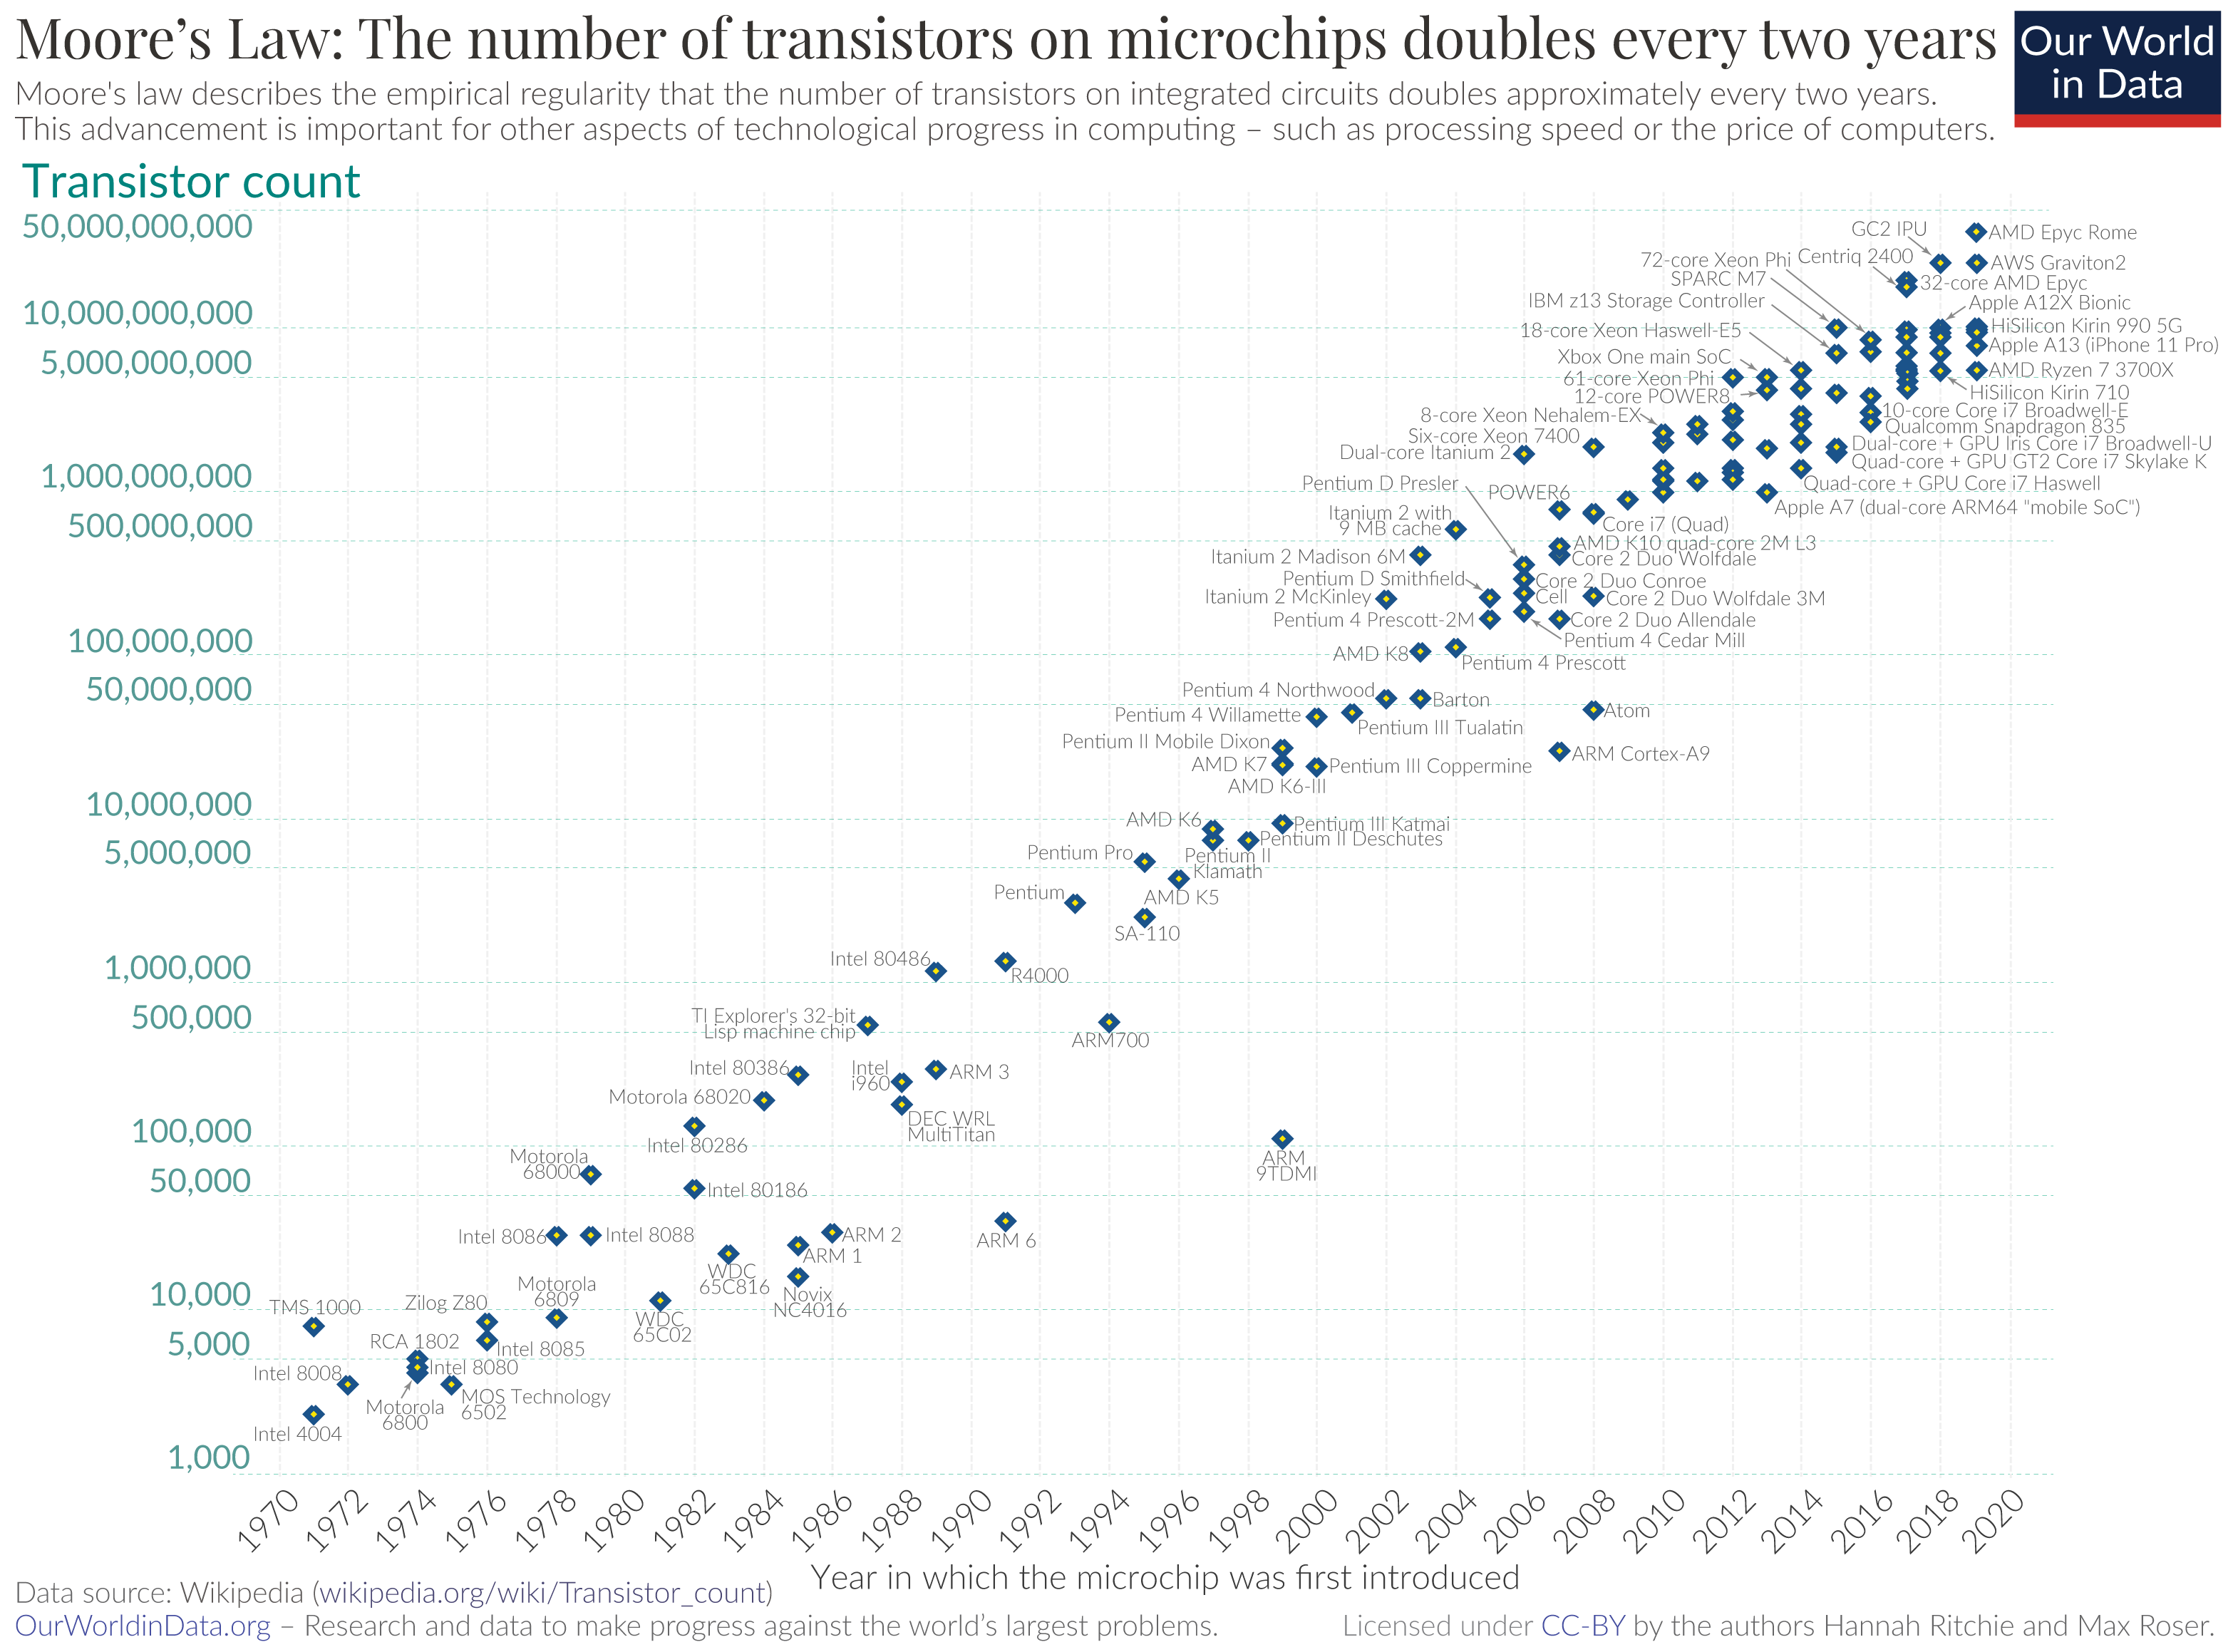
\includegraphics[width=0.65\linewidth]{figures/cpu_transistor_counts.png}
\end{figure}
\end{frame}

\begin{frame}{Decrease in Cost Per FLOPS}
\begin{figure}
  \centering
  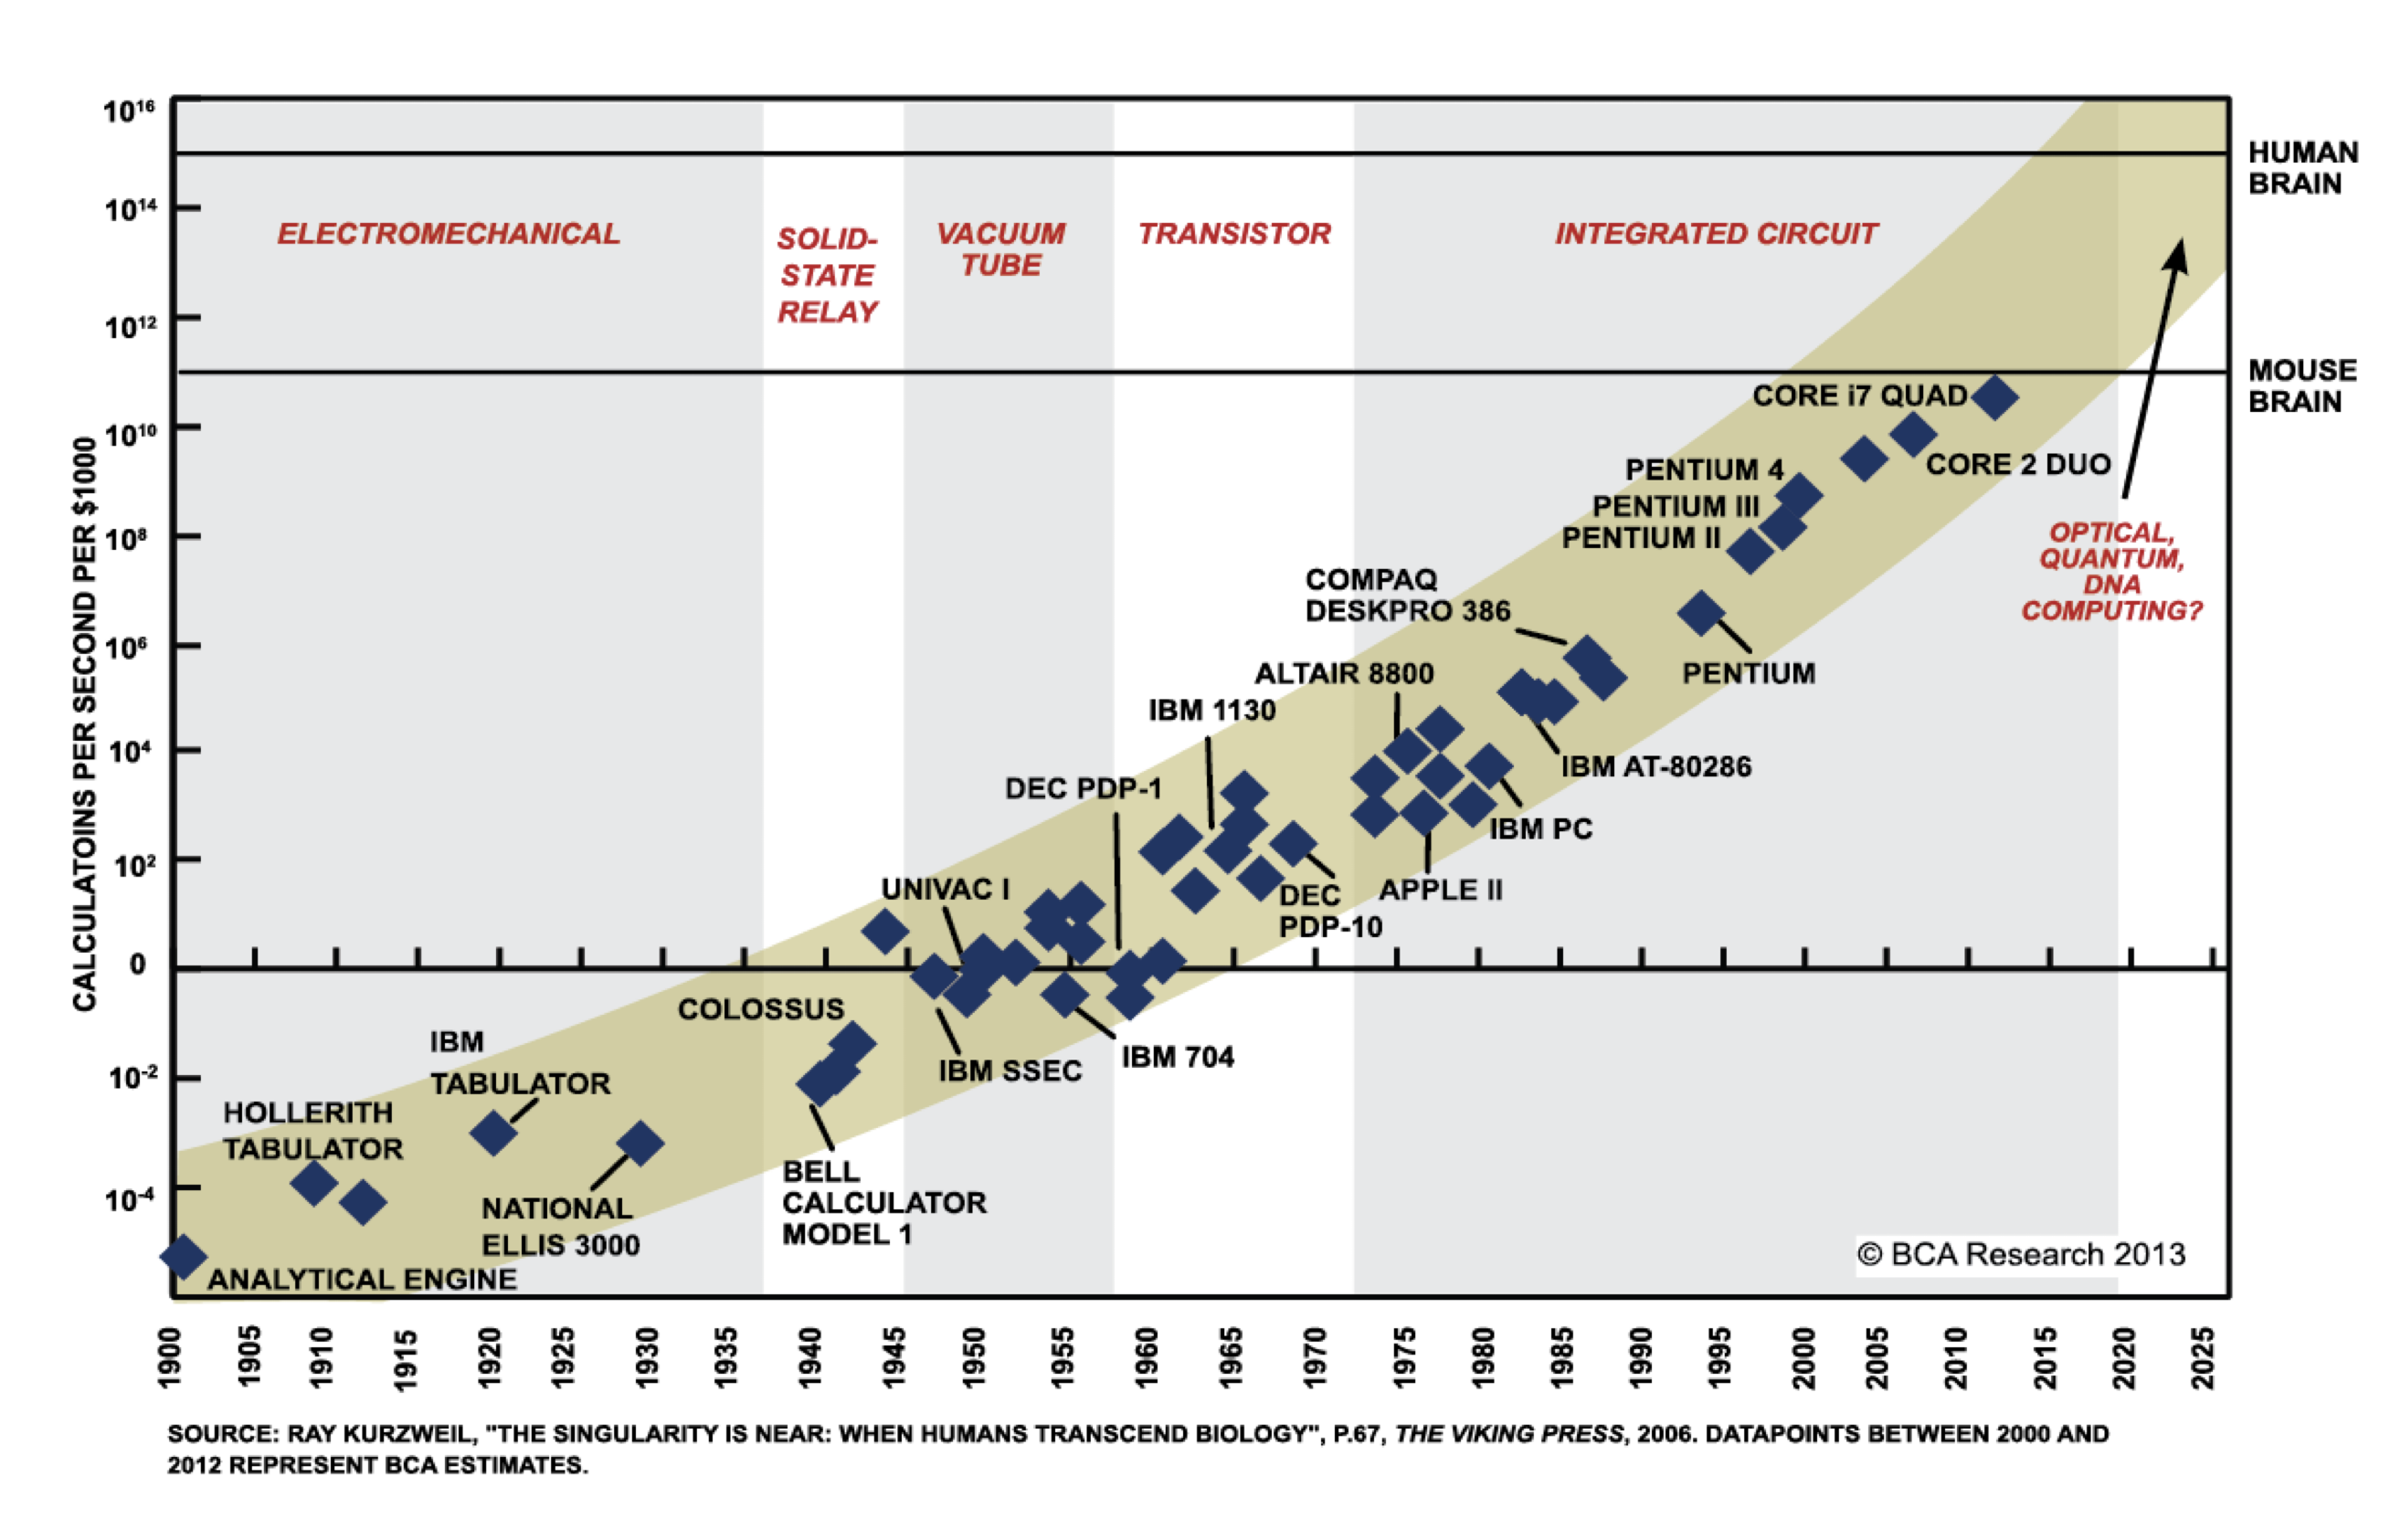
\includegraphics[width=0.65\linewidth]{figures/compute_cost.png}
\end{figure}
\end{frame}

\begin{frame}{Additional Problems}
\begin{itemize}
\item Growing performance discrepancy between processing units and data storage
\begin{itemize}
\item 40\% processor performance improvement per year
\item 10\% RAM performance improvement per year
\end{itemize}
\item Discrepancy leads to memory-bound programs
\begin{itemize}
\item CPU spends more and more time idle, waiting on data from
\end{itemize}
\item Many simulations require incredible amounts of memory to achieve high-accuracy solutions (PDE, MD, QM, etc.)
\begin{itemize}
\item These cannot fit on a single computer alone
\end{itemize}
\end{itemize}
\end{frame}

\begin{frame}{The Parallel Solution}
\begin{itemize}
\item Using multiple processing units (cores, etc.) simultaneously to perform a computation
\item Use multiple computers to store data for large problems
\item Essentially all modern CPUs have multiple cores
\end{itemize}
\end{frame}

\begin{frame}{Parallel Programming}
\centering
``I know how to make 4 horses pull a cart - I don't know how to make 1024
chickens do it.''\\Enrico Clementi
\end{frame}

\begin{frame}{What is High-Performance Computing}
\centering
High performance computing (HPC) is the use of computing resources that are
significantly more powerful than what is commonly available.

As such, it's always a moving target.
\end{frame}

\begin{frame}{Supercomputer Types}
\begin{columns}
\begin{column}{0.5\textwidth}
\begin{itemize}
\item Single processor
\item Shared Memory Parallel (SMP)
\item Massively Parallel Processors
\item Constellations
\item Clusters
\end{itemize}
\end{column}
\begin{column}{0.5\textwidth}
\begin{center}
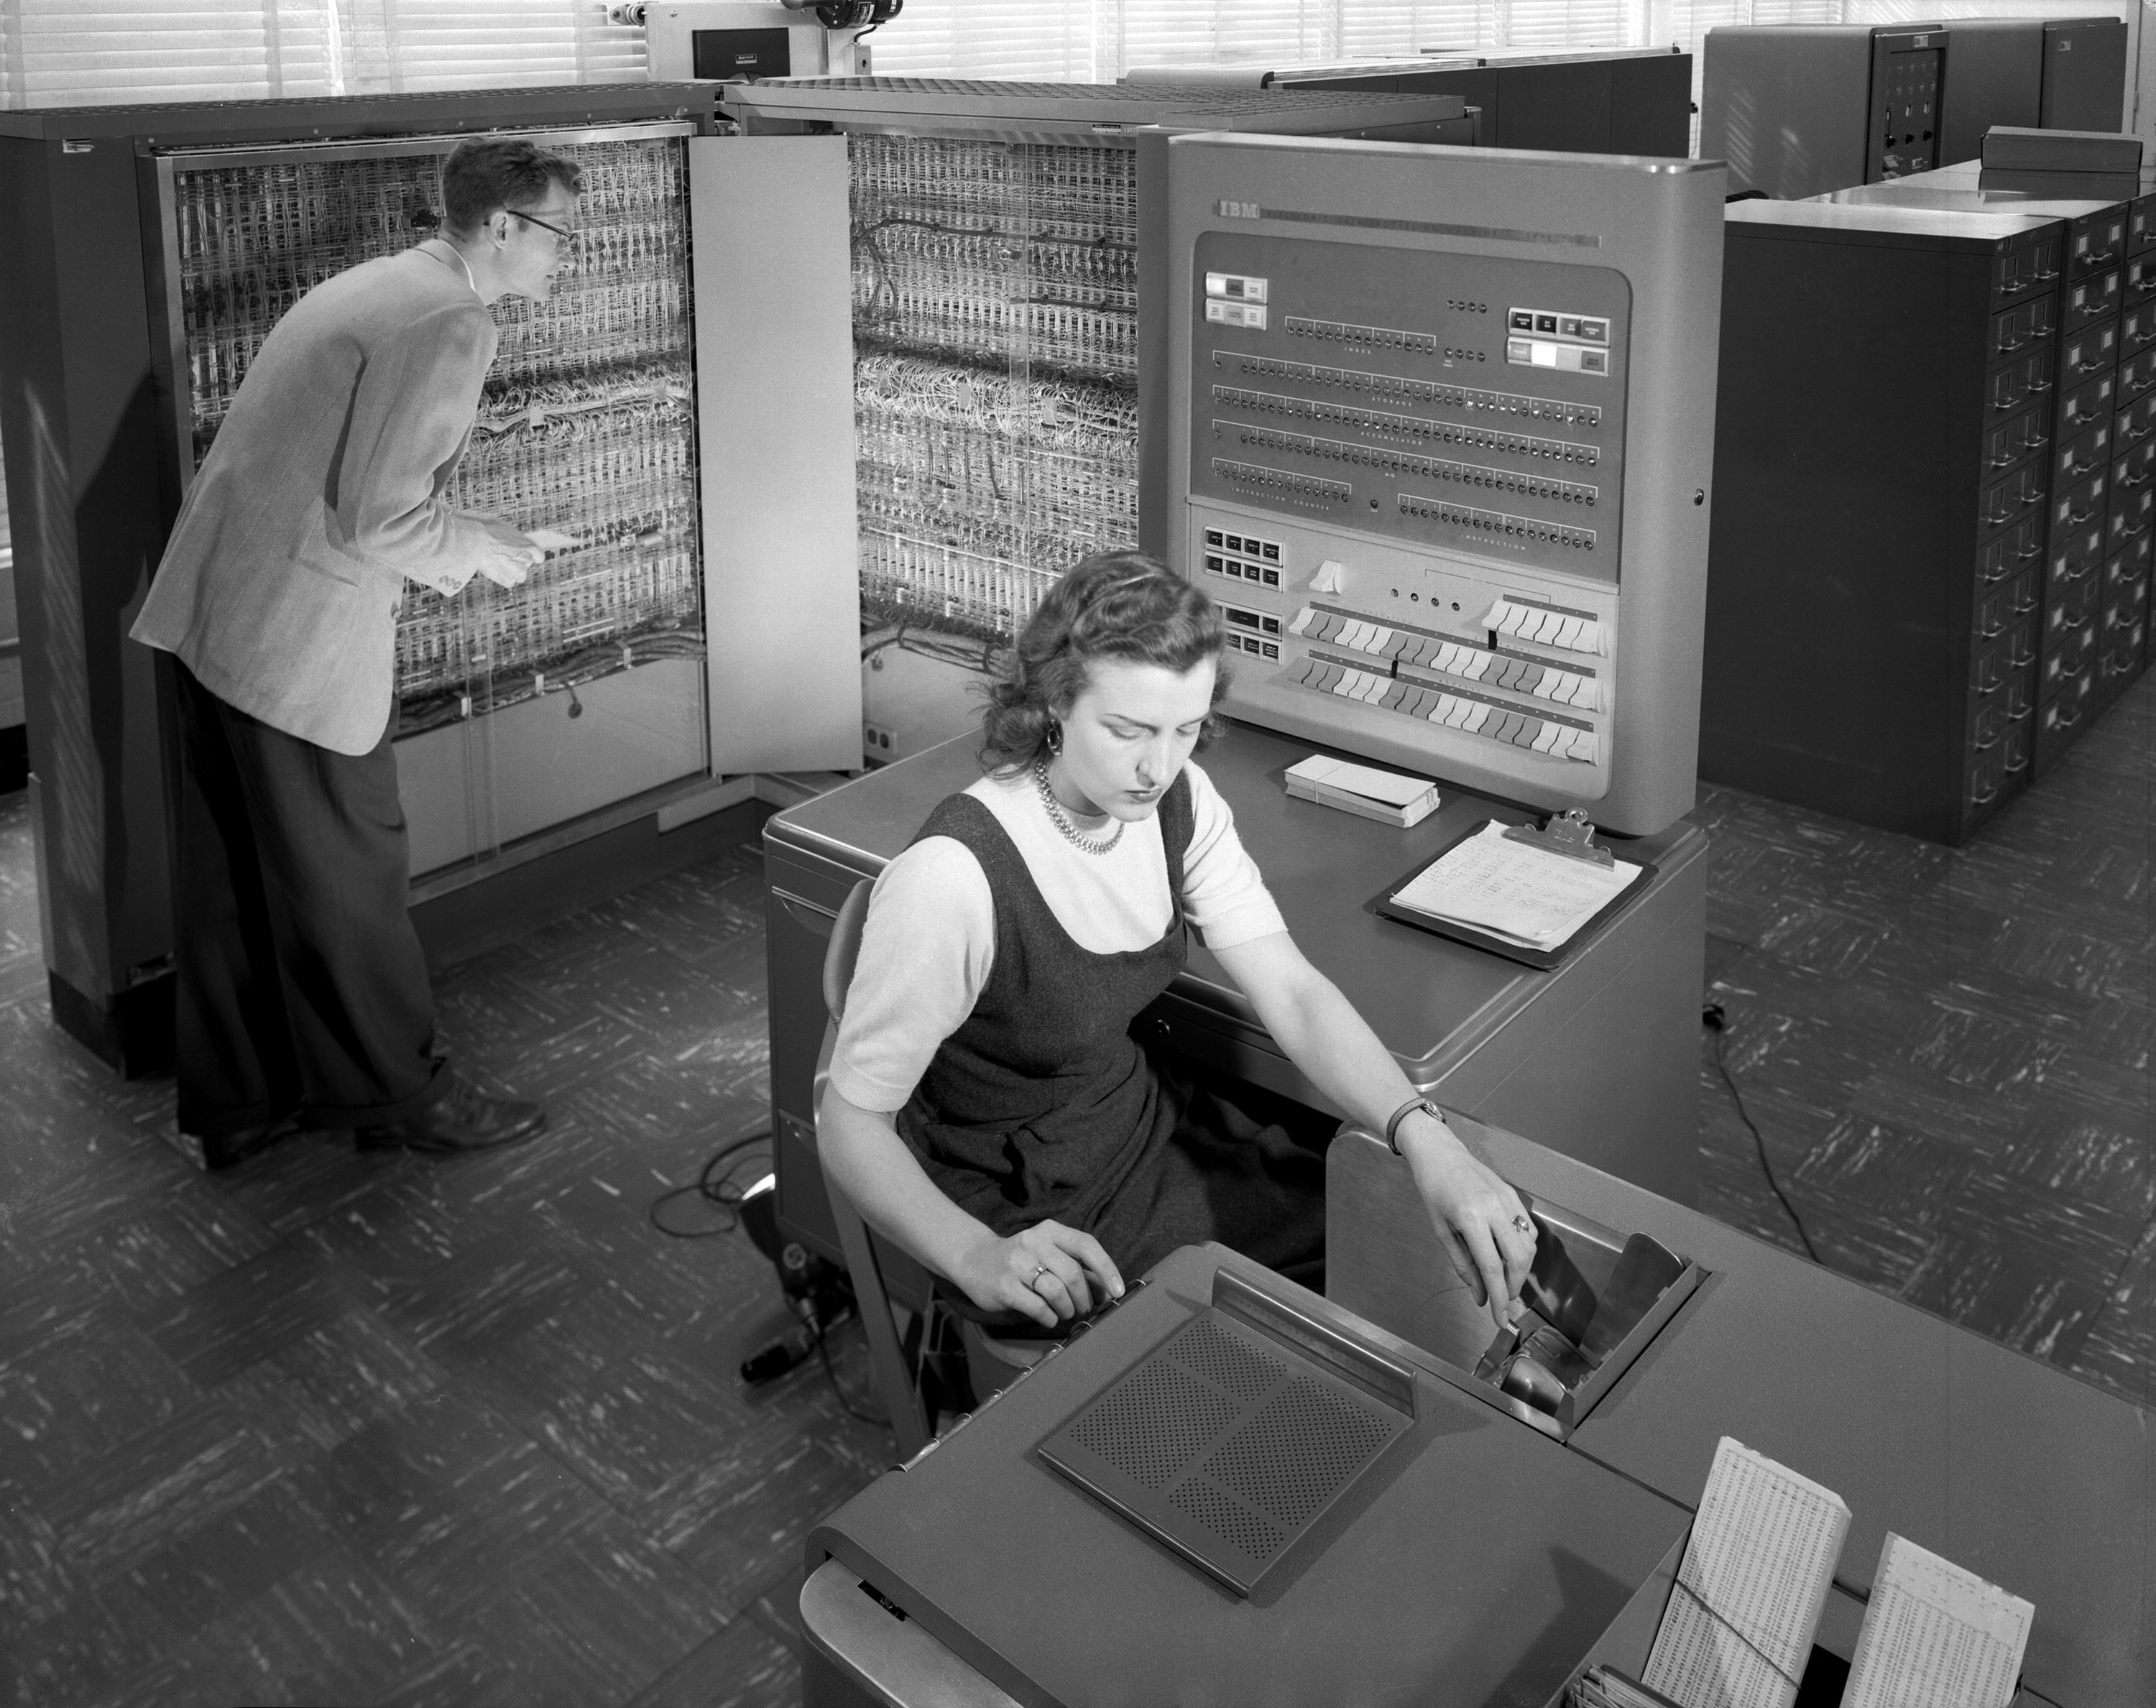
\includegraphics[width=\textwidth]{figures/mainframe.jpg}
\end{center}
\end{column}
\end{columns}
\end{frame}

\begin{frame}{History of Parallel Architectures}
\begin{columns}
\begin{column}{0.5\textwidth}
\begin{center}
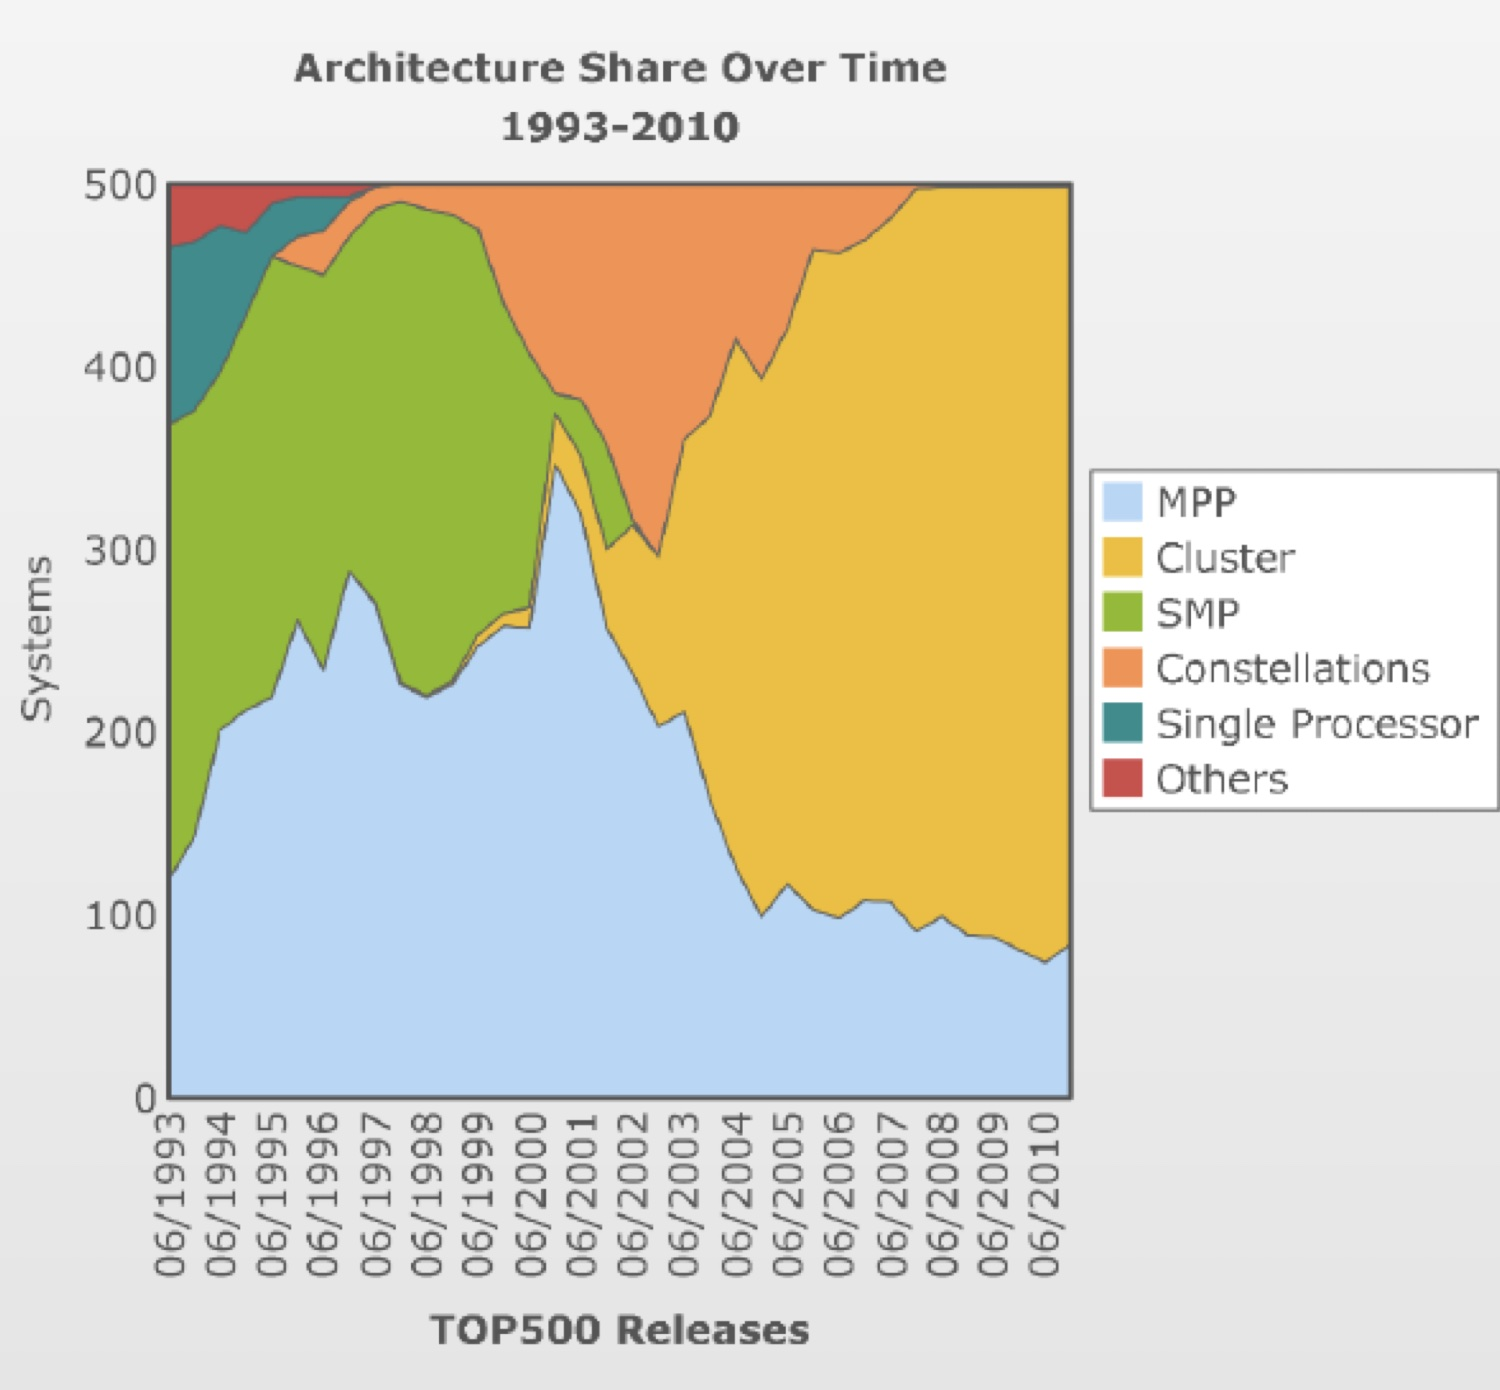
\includegraphics[width=\textwidth]{figures/top500_architecture.jpg}
\end{center}
\end{column}
\begin{column}{0.5\textwidth}
\begin{center}
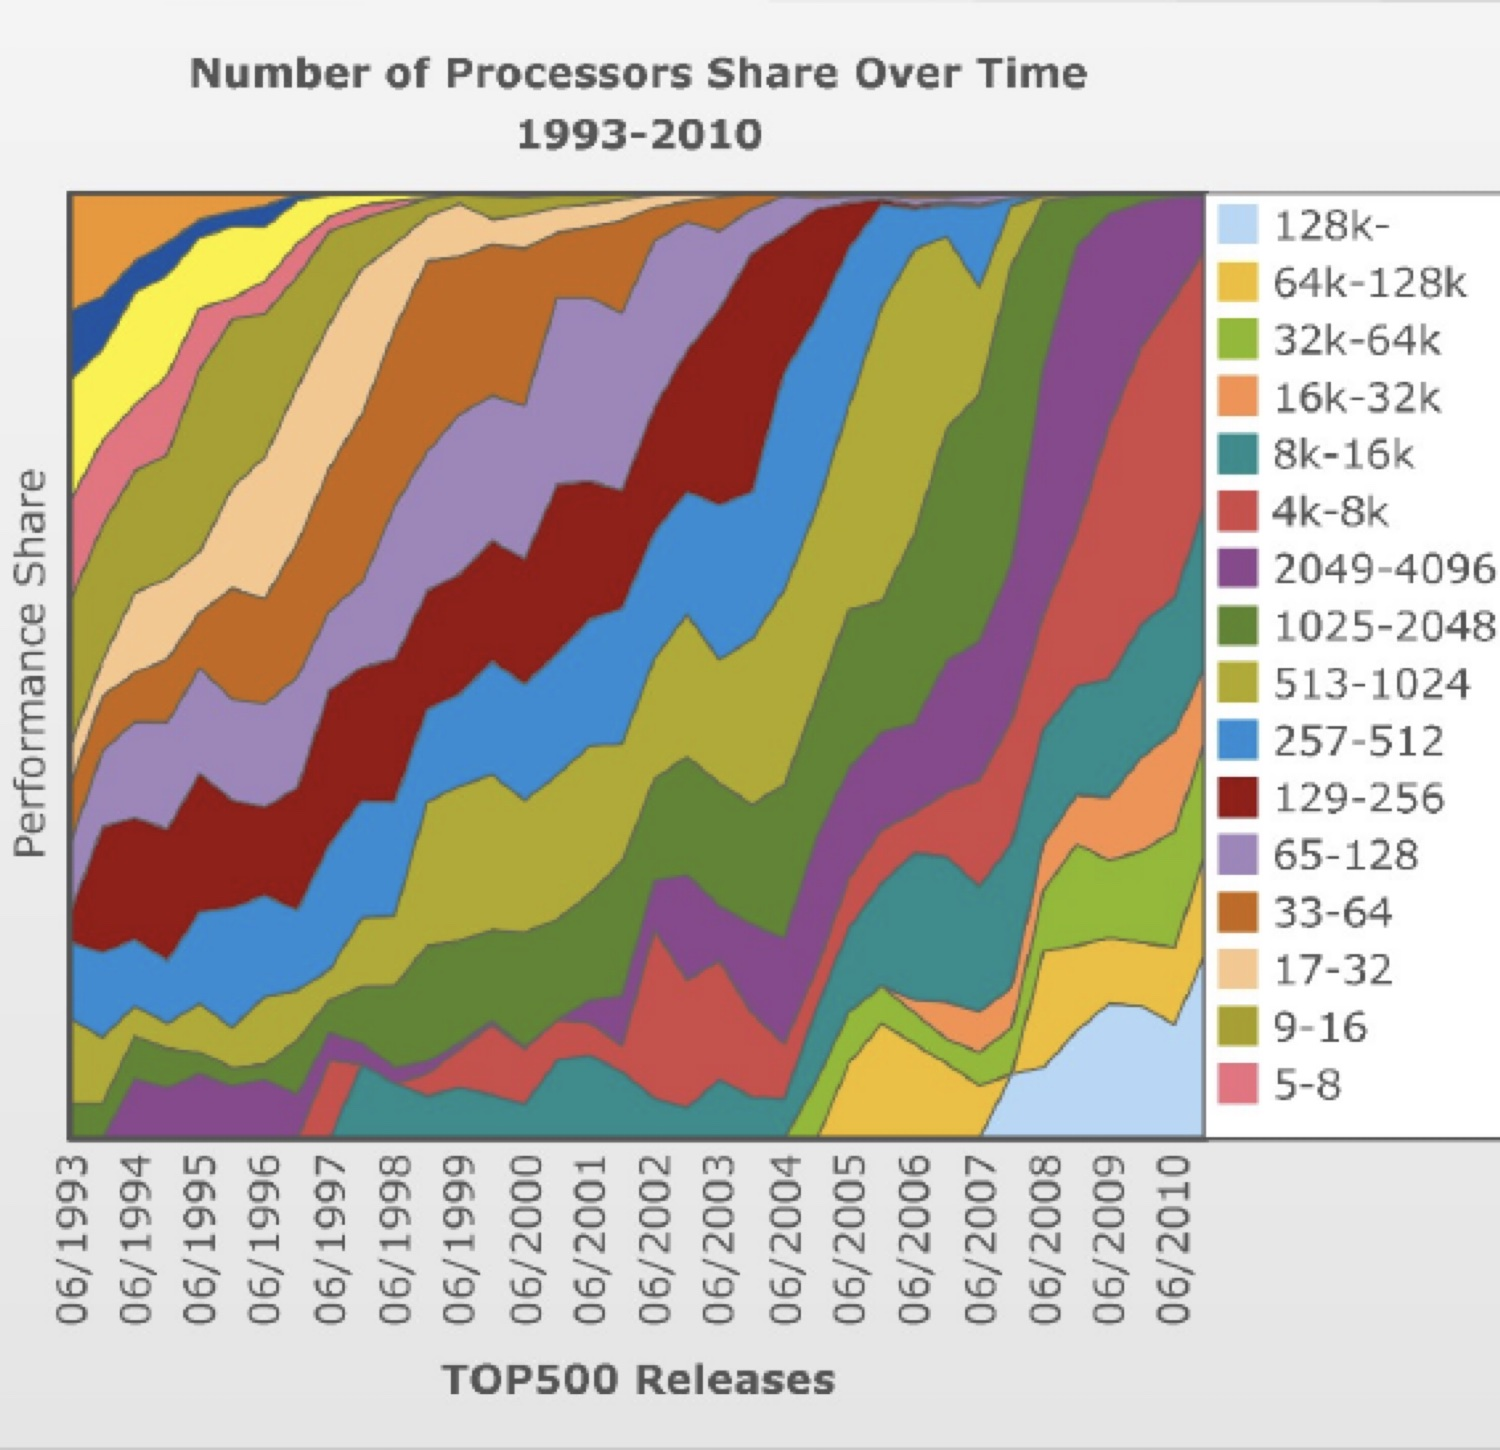
\includegraphics[width=\textwidth]{figures/top500_core_count.jpg}
\end{center}
\end{column}
\end{columns}
\end{frame}

\begin{frame}{Flynn’s Parallel Architecture Taxonomy}
\begin{columns}
\begin{column}{0.5\textwidth}
\begin{itemize}
\item Single/multiple instruction streams
\begin{itemize}
\item Number of types of instructions to be performed at once
\end{itemize}
\item Single/multiple data streams
\begin{itemize}
\item Number of data streams to be operated on at once
\end{itemize}
\item Most modern parallel computers are MIMD
\item SIMD was popular until 1990s
\item MISD never used to large extent
\end{itemize}
\end{column}
\begin{column}{0.5\textwidth}
\begin{center}
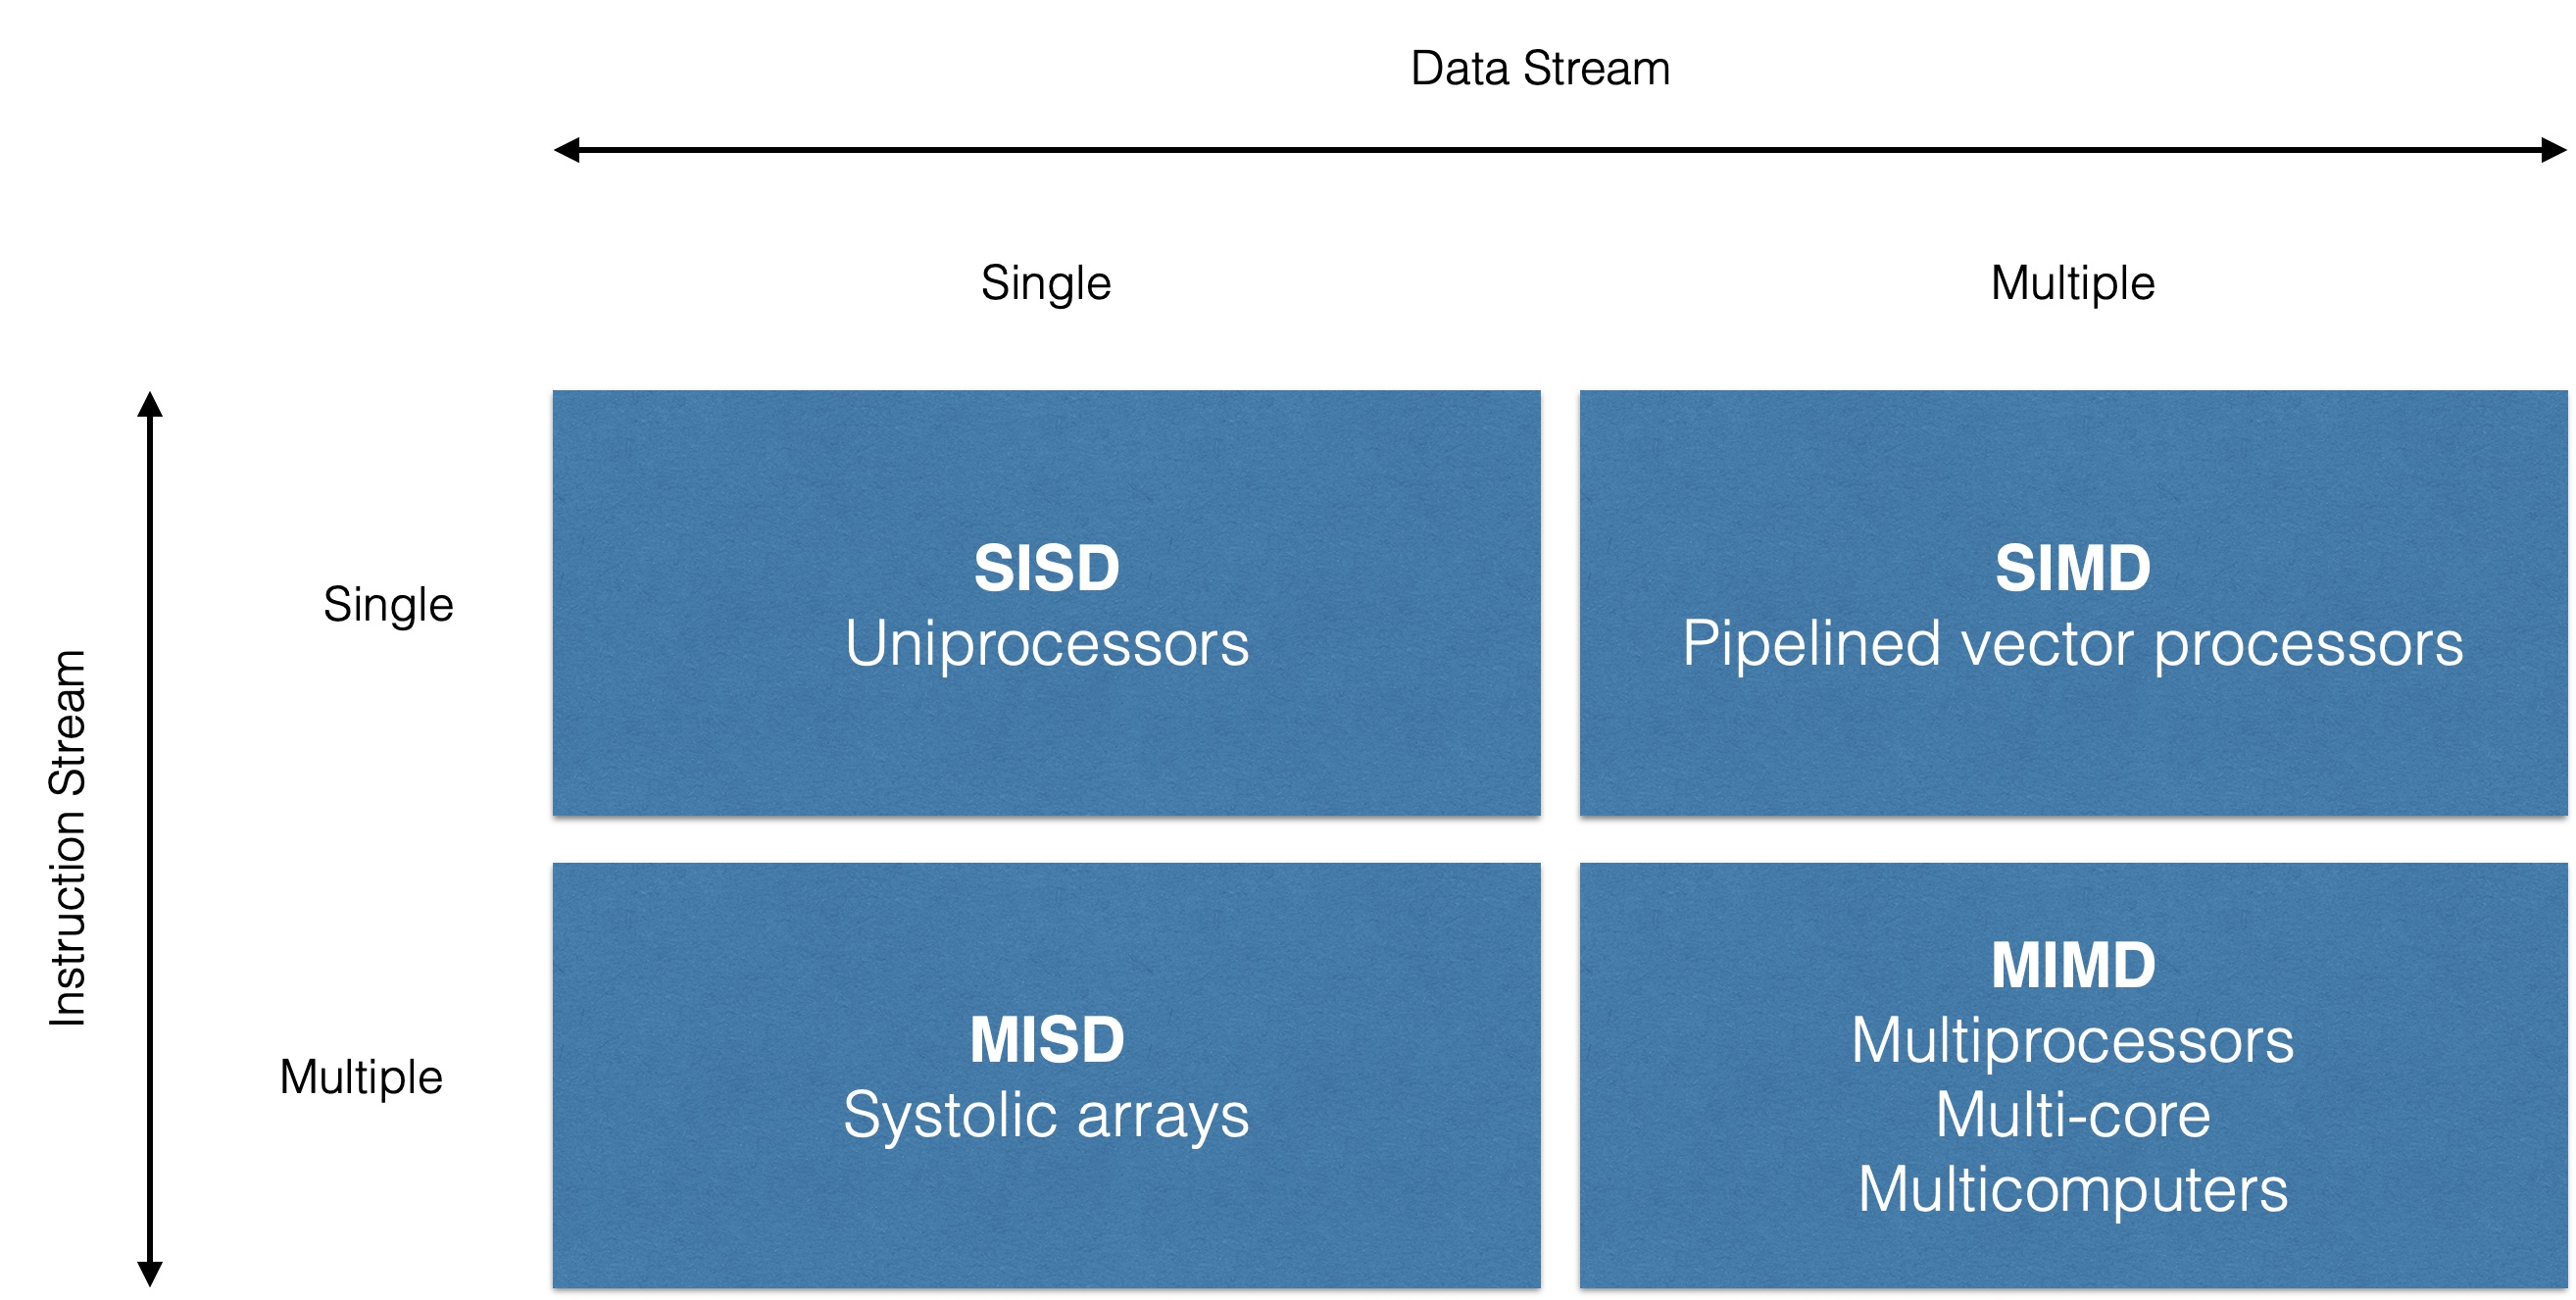
\includegraphics[width=\textwidth]{figures/flynn_taxonomy.jpg}
\end{center}
\end{column}
\end{columns}
\end{frame}

\begin{frame}{Multicomputer Architecture}
\begin{center}
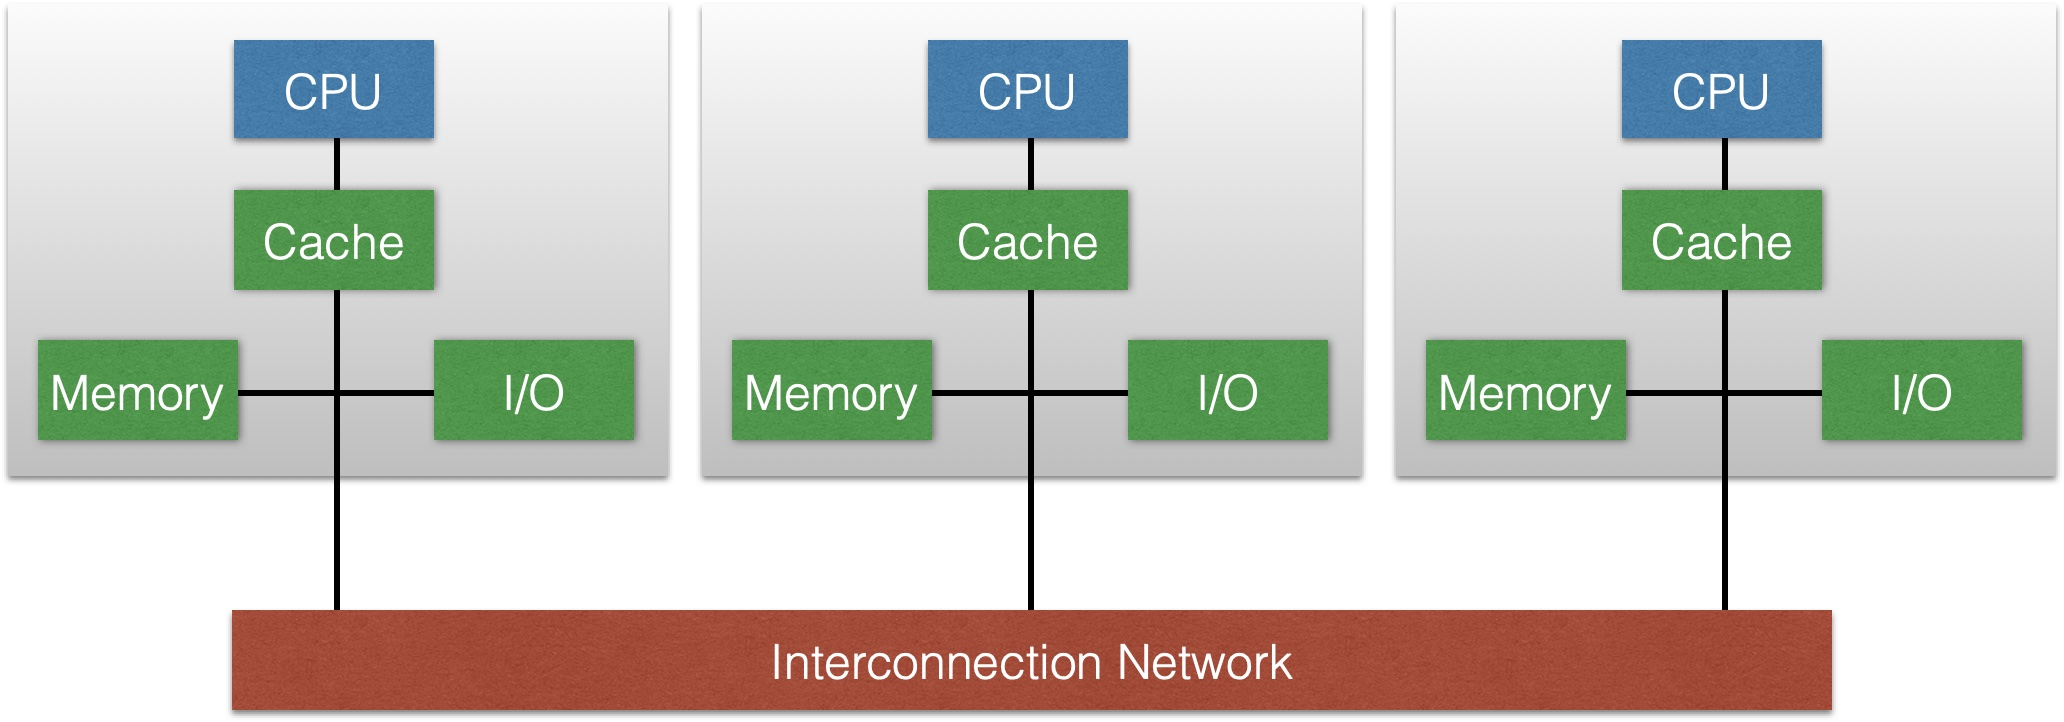
\includegraphics[scale=0.25]{figures/cluster_interconnect.jpg}
\end{center}
\begin{itemize}
\item Each processor only has direct access to its own local memory address space
\begin{itemize}
\item The same address on different processors refers to different memory locations
\end{itemize}
\item Processors interact with one another through passing messages
\item Commercial multicomputers typically provide a custom switching network to
      provide low-latency, high-bandwidth access between processors
\end{itemize}
\end{frame}

\begin{frame}{Multicomputer Architecture}
\begin{itemize}
\item Commodity clusters are build using commodity computers and switches/LANs
\item Less costly than SMP's
\item Increased latency/decreased bandwidth between CPUs
\item Theoretically extensible to arbitrary processor counts
\item Software becomes complicated
\item Networking gets expensive
\end{itemize}
\end{frame}

\begin{frame}{Cluster Storage Resources}
\begin{columns}
\begin{column}{0.5\textwidth}
\begin{itemize}
\item Usually there is an inverse relationship between storage amount and speed
\item Clusters and applications can distort the standard order
\begin{itemize}
\item Aggregation, e.g. RAID
\item Network optimization to a specific topology
\item Applications can be configured and built for specific hardware
\item New hardware technologies
\end{itemize}
\end{itemize}
\end{column}
\begin{column}{0.5\textwidth}
\begin{center}
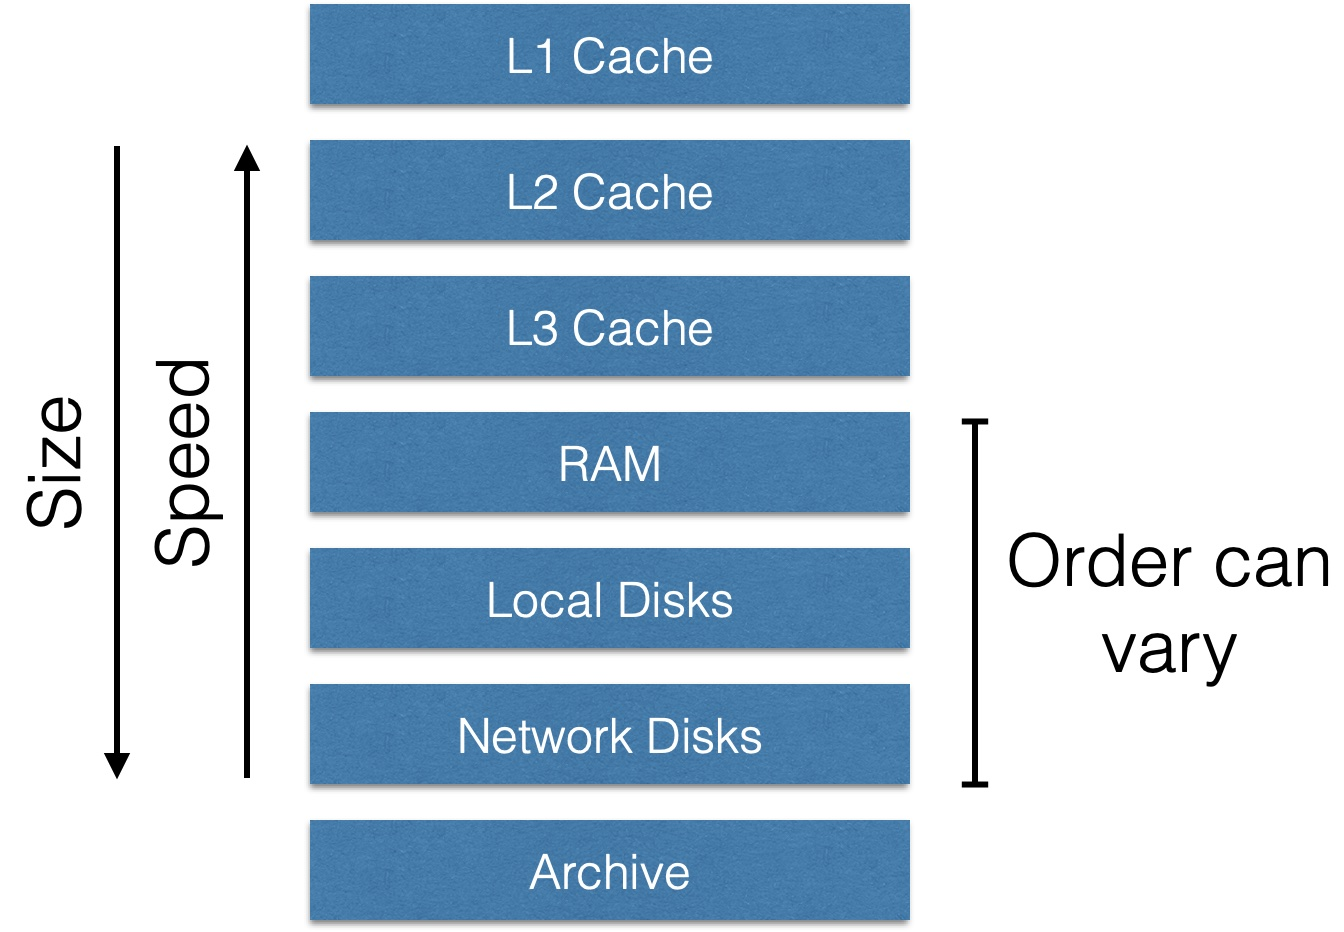
\includegraphics[width=\textwidth]{figures/storage_hierarchy.jpg}
\end{center}
\end{column}
\end{columns}
\end{frame}

\begin{frame}{Cluster Super Computers}
\begin{figure}
  \centering
  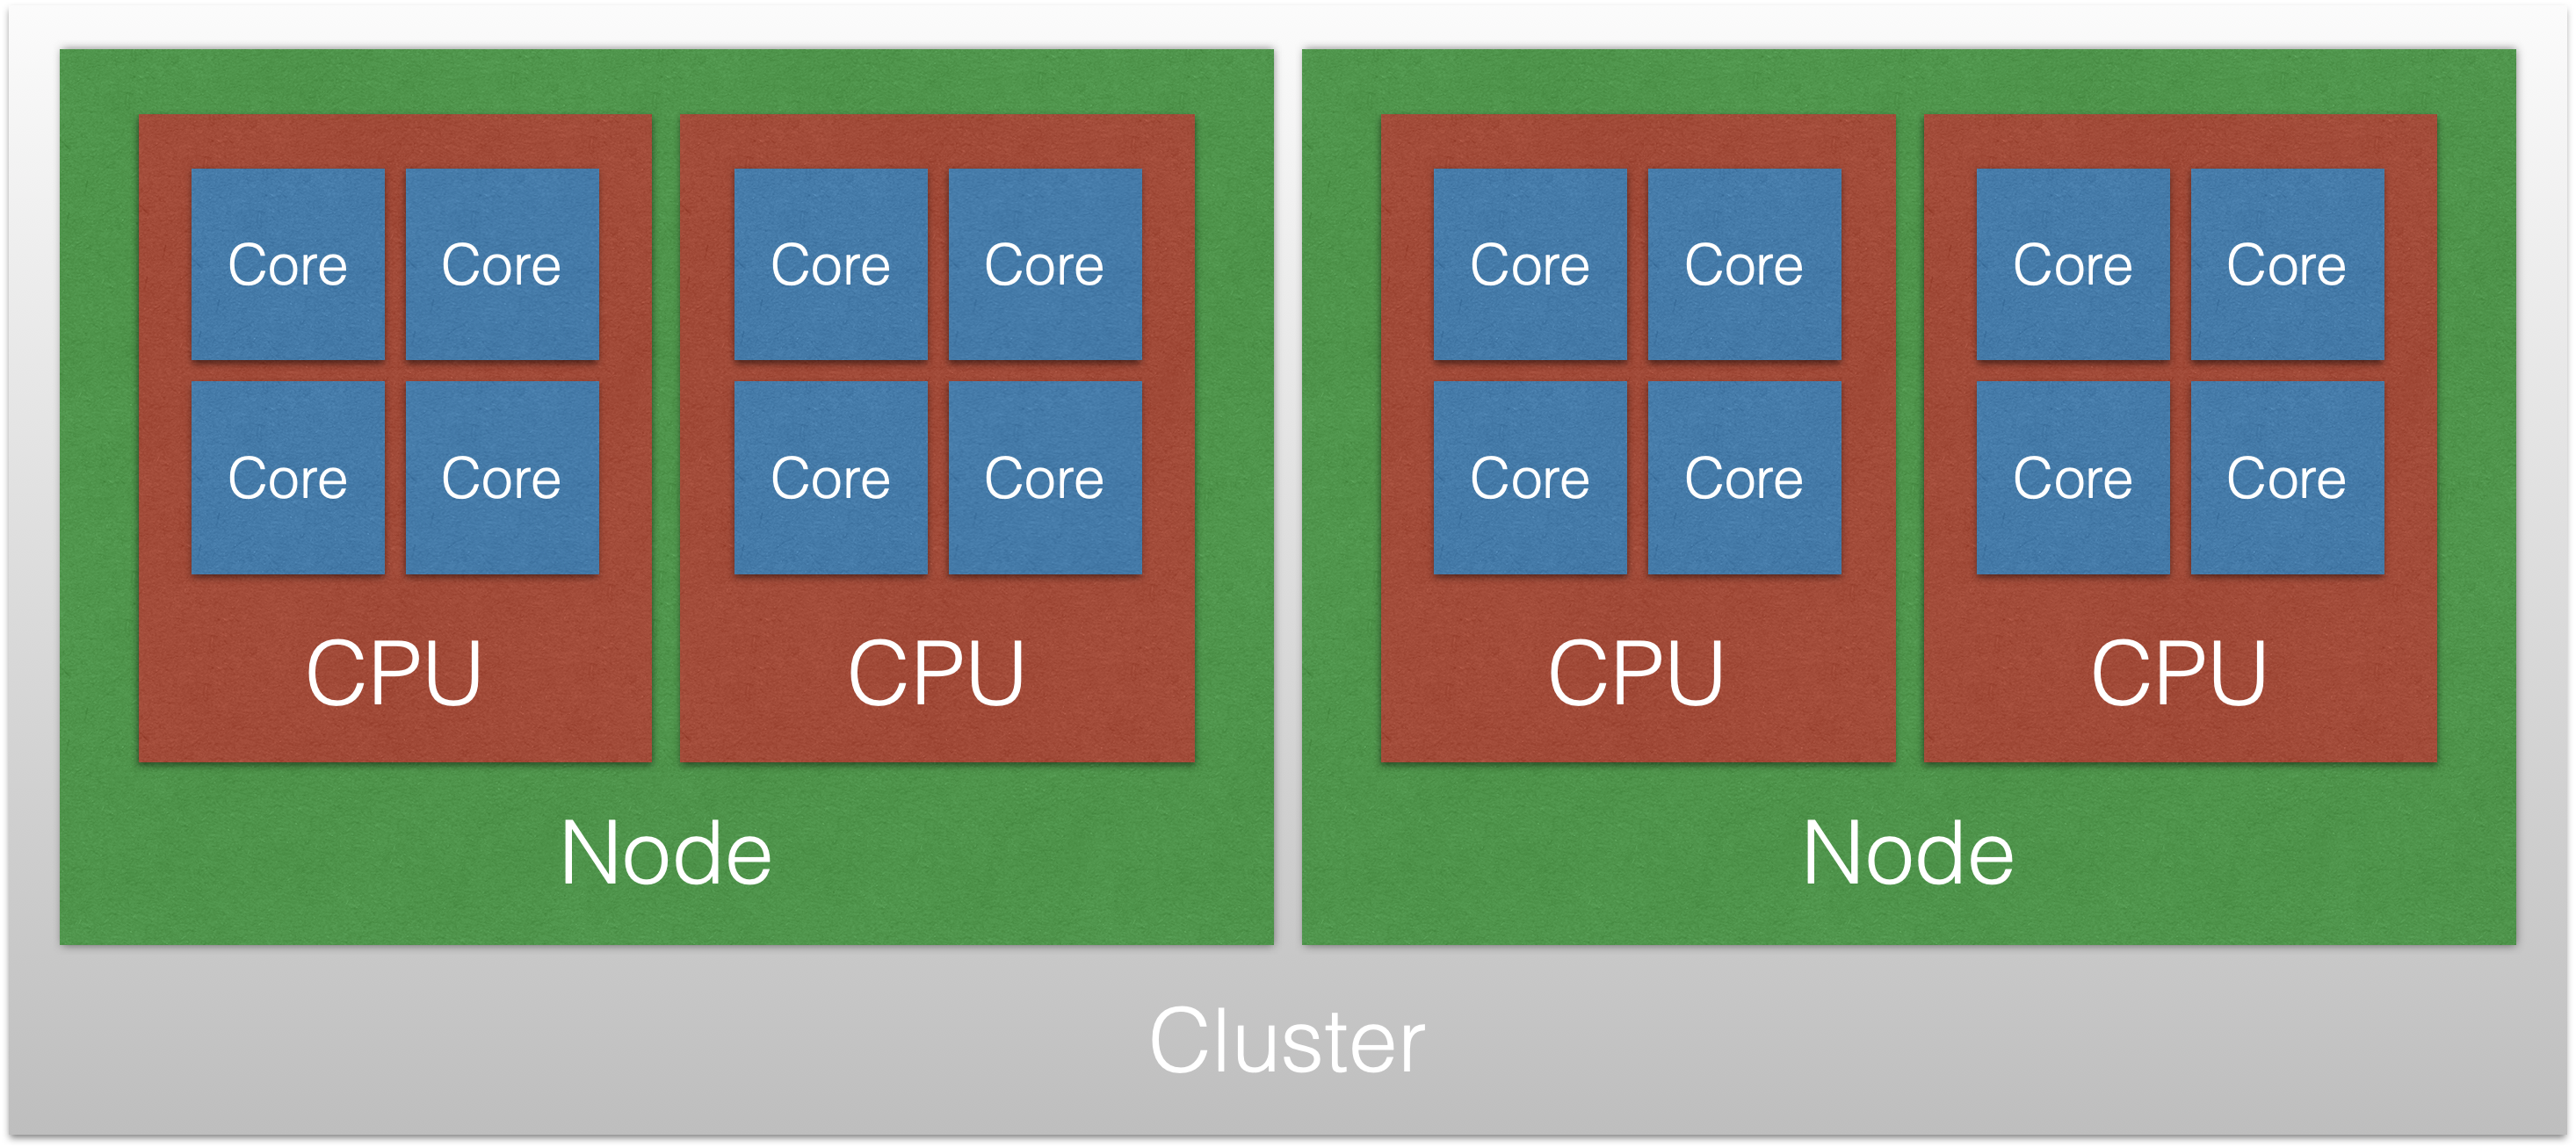
\includegraphics[width=0.75\linewidth]{figures/cluster.png}
  \caption{A cluster is a collection of individual computers networked together. Applications can be configured to run on all available compute resources.}
\end{figure}
\end{frame}

\section{SMU HPC Clusters}

\begin{frame}{ManeFrame II (M2) Node Types}
\begin{table}
\tiny
\begin{tabular}{lllll}
\toprule
Type & Quantity & Cores & Memory [GB] & Additional Resources\\
\midrule
Standard-Memory & 176 & 36 & 256 & \\
Medium-Memory-1 & 35 & 36 & 768 & \\
Medium-Memory-2 & 4 & 24 & 768 & 3 TB SSD local scratch\\
High-Memory-1 & 5 & 36 & 1,536 & \\
High-Memory-2 & 6 & 40 & 1,536 & 3 TB SSD local scratch\\
GPGPU-1 & 36 & 36 & 256 & NVIDIA P100 GPU has 3,584 CUDA cores and 16 GB CoWoS\\
MIC-1 & 36 & 64 & 384 & 16 GB of high bandwidth (400 GB/s) stacked memory\\
VDI & 5 & 36 & 256 & NVIDIA Quadro M5000 GPU\\
v100x8 & 3 & 36 & 768 & 8 NVIDIA V100 GPUs with 5,120 CUDA cores and 32 GB CoWoS\\
Faculty Partner Nodes & 3 &  &  & Various research specific NVIDIA GPU configurations\\
\midrule
ManeFrame II & 354 & 11,276 & 120 TB & 2.8 PB storage and InfiniBand network\\
\bottomrule
\end{tabular}
\end{table}
\end{frame}

\begin{frame}{NVIDIA DGX SuperPOD (MP)}
\begin{columns}
\begin{column}{0.5\textwidth}
\begin{itemize}
\item 20 NVIDIA DGX nodes
\item 8 NVIDIA A100 80 GB GPUs per node
\item Dual AMD Epyc 7742 2.25 GHz 64-core ``Rome'' processors per node
\item 200 Gb/s \(\times\) 10 NVIDIA/Mellanox InfiniBand networking
\end{itemize}
\end{column}
\begin{column}{0.5\textwidth}
\begin{center}
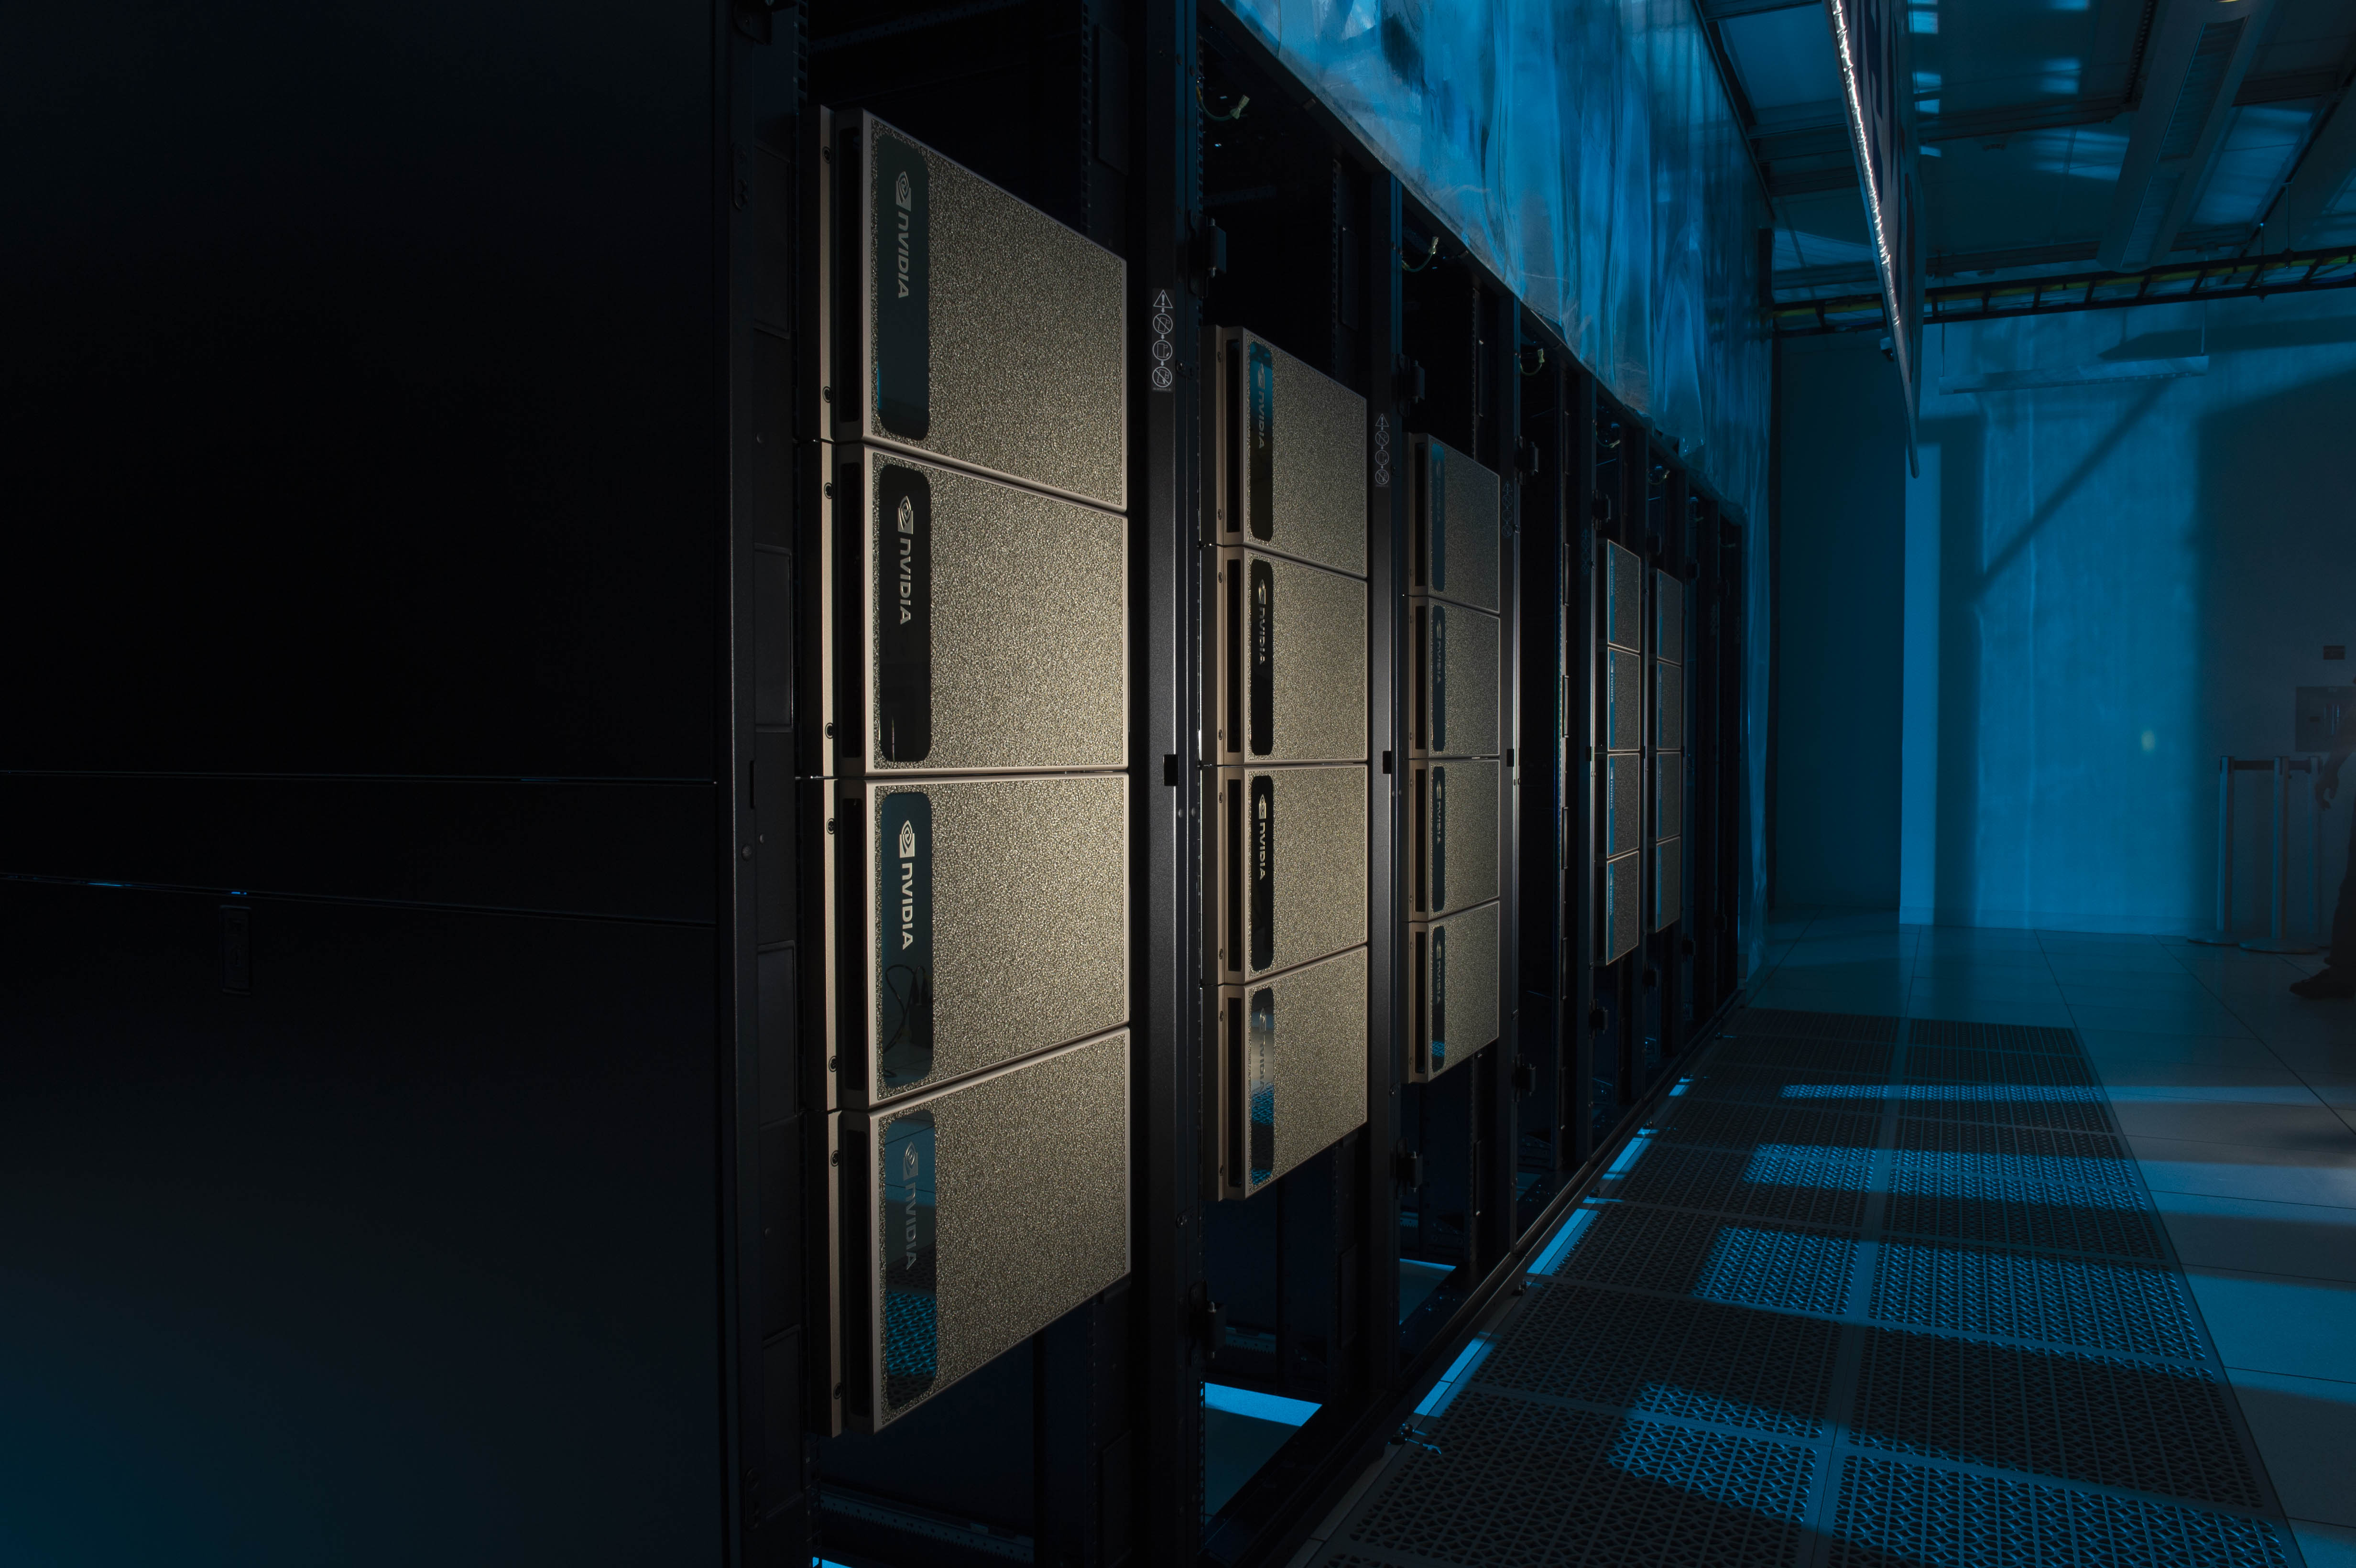
\includegraphics[width=\textwidth]{figures/superpod.jpg}
\end{center}
\end{column}
\end{columns}
\end{frame}

\begin{frame}{SMU HPC File Systems}
\begin{description}
\item[\$HOME]
\begin{itemize}
  \item Default file system when logging into M2, e.g. \mintinline{sh}{/users/$USER}.
  \item Space should be used to write, edit, compile programs, and job submission scripts, etc.
  \item Restricted by quotas (200 GB) and backed-up.
\end{itemize}
\item[\$WORK]
\begin{itemize}
  \item Long term storage at \mintinline{sh}{/work/users/$USER}.
  \item Restricted by quotas (8 TB) and not backed-up.
\end{itemize}
\item[\$SCRATCH]
\begin{itemize}
 \item Scratch space at \mintinline{sh}{/scratch/users/$USER}.
 \item Treat \$SCRATCH as a volatile file system that is not backed-up.
\end{itemize}
\end{description}
\end{frame}

\begin{frame}{Unversity Data Center (UDC)}
\begin{columns}
\begin{column}{0.5\textwidth}
\begin{center}
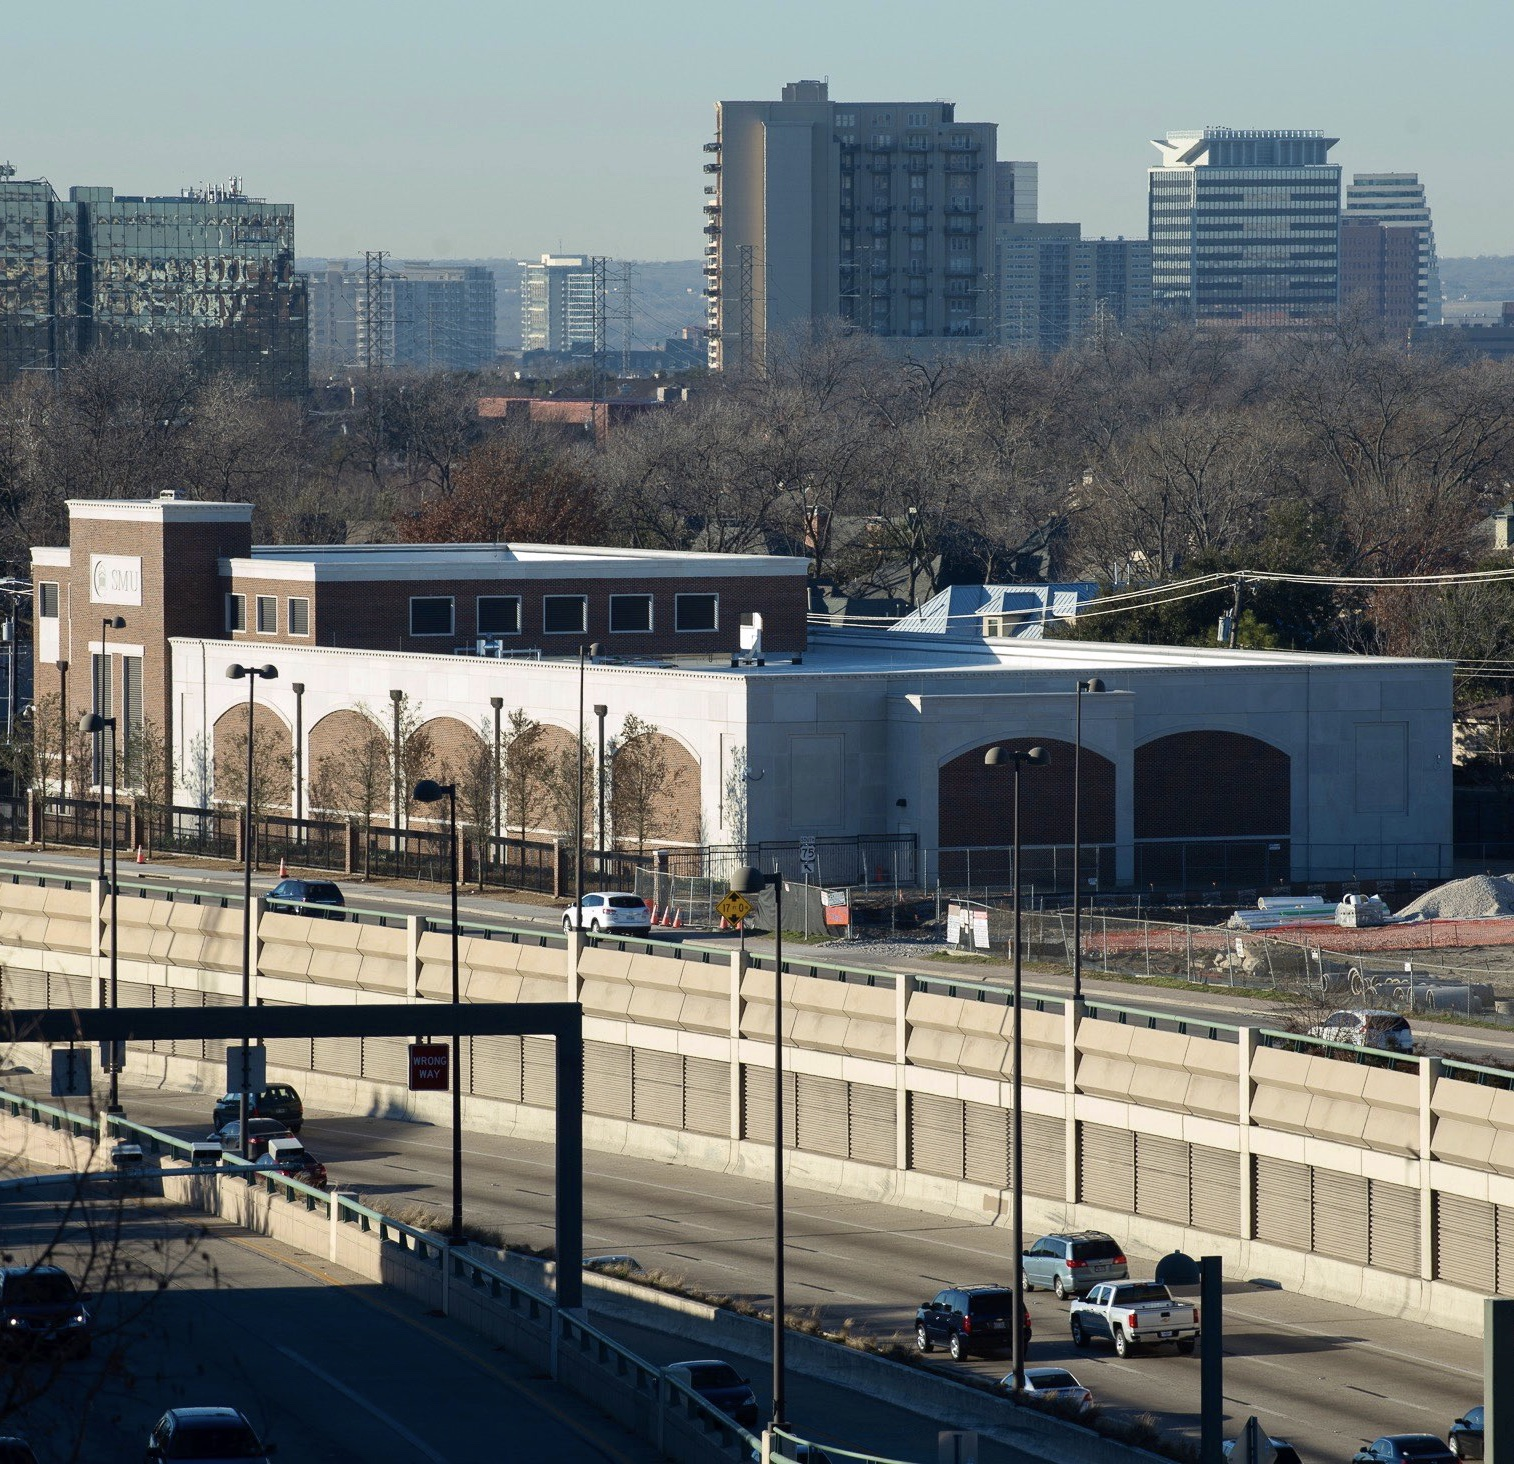
\includegraphics[width=\textwidth]{figures/udc_1.jpg}
\end{center}
\end{column}
\begin{column}{0.5\textwidth}
\begin{center}
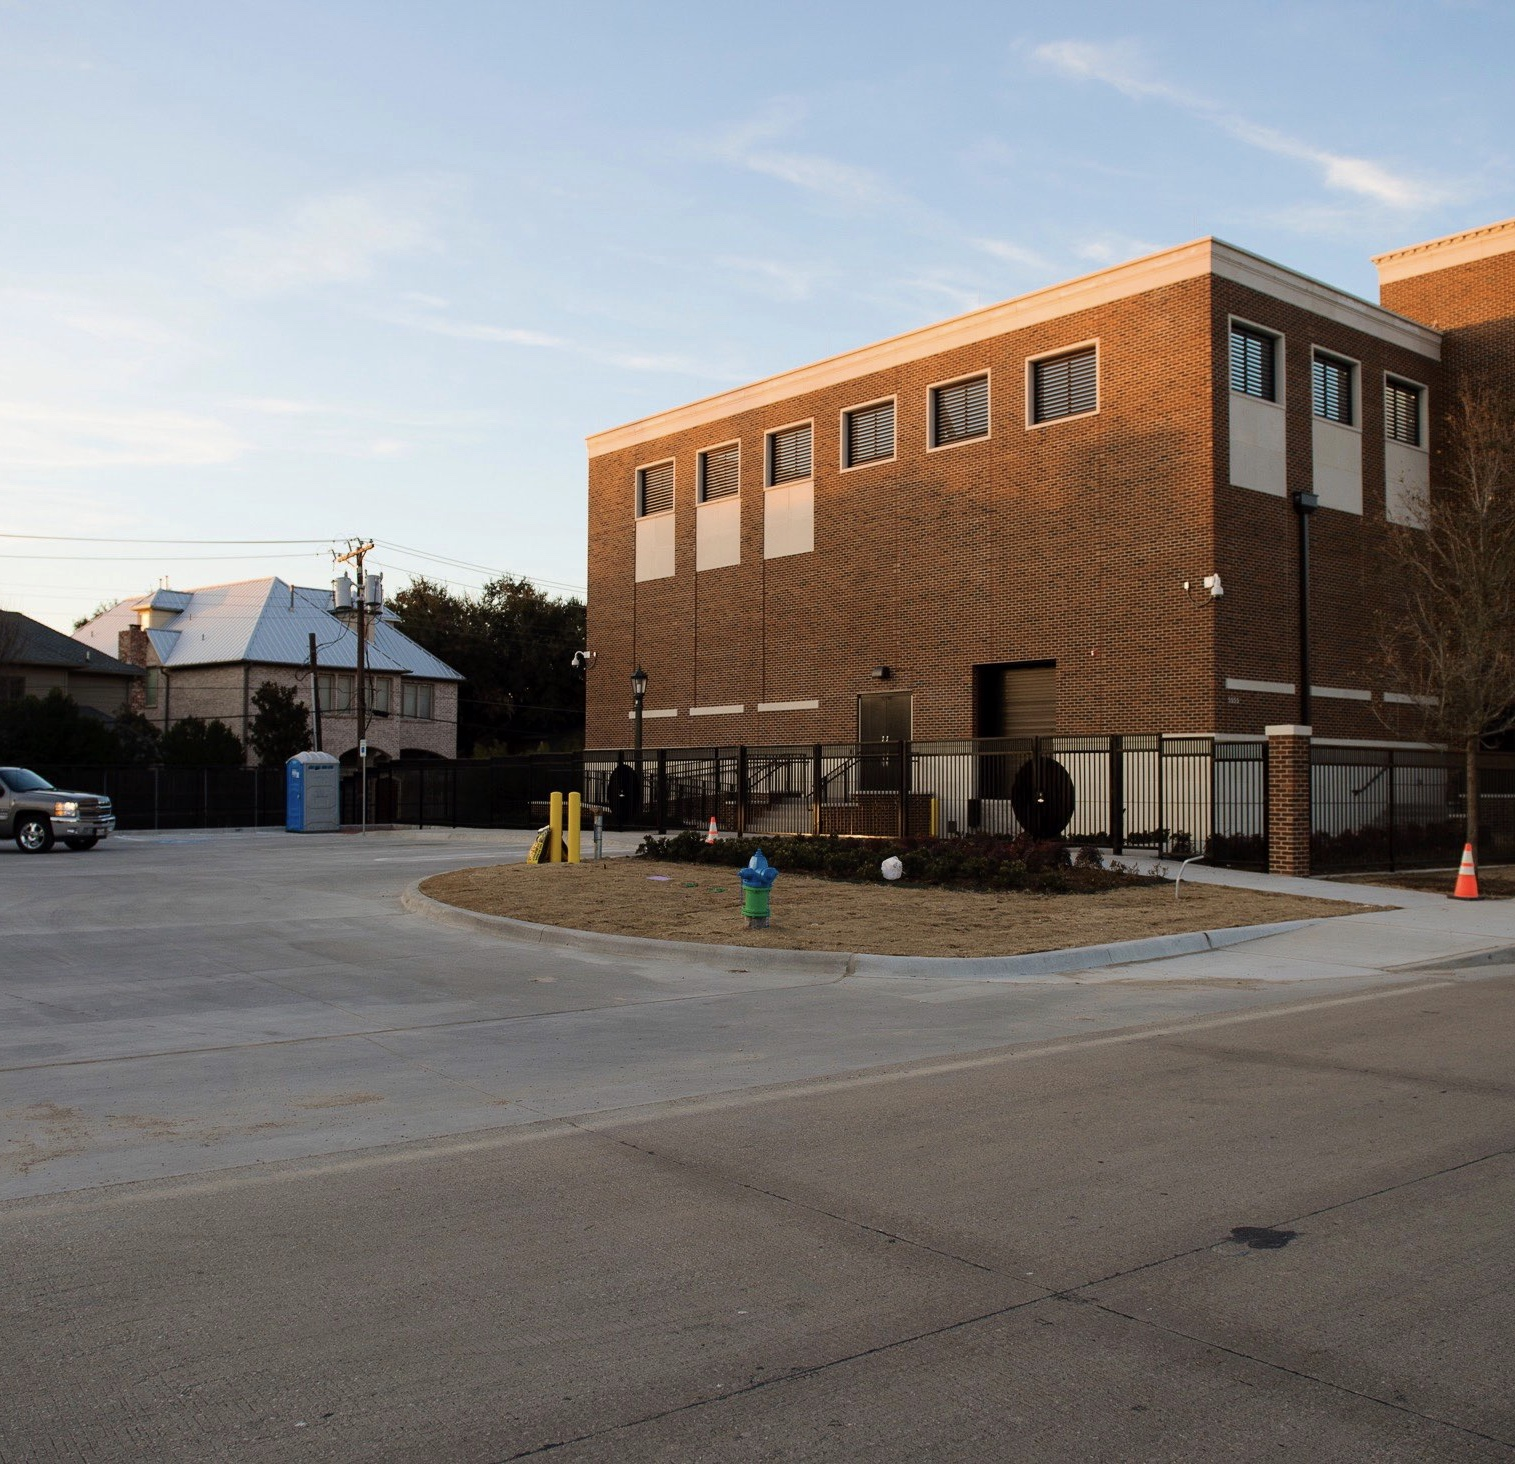
\includegraphics[width=\textwidth]{figures/udc_2.jpg}
\end{center}
\end{column}
\end{columns}
\end{frame}

\begin{frame}{ManeFrame II (M2)}
\begin{columns}
\begin{column}{0.5\textwidth}
\begin{center}
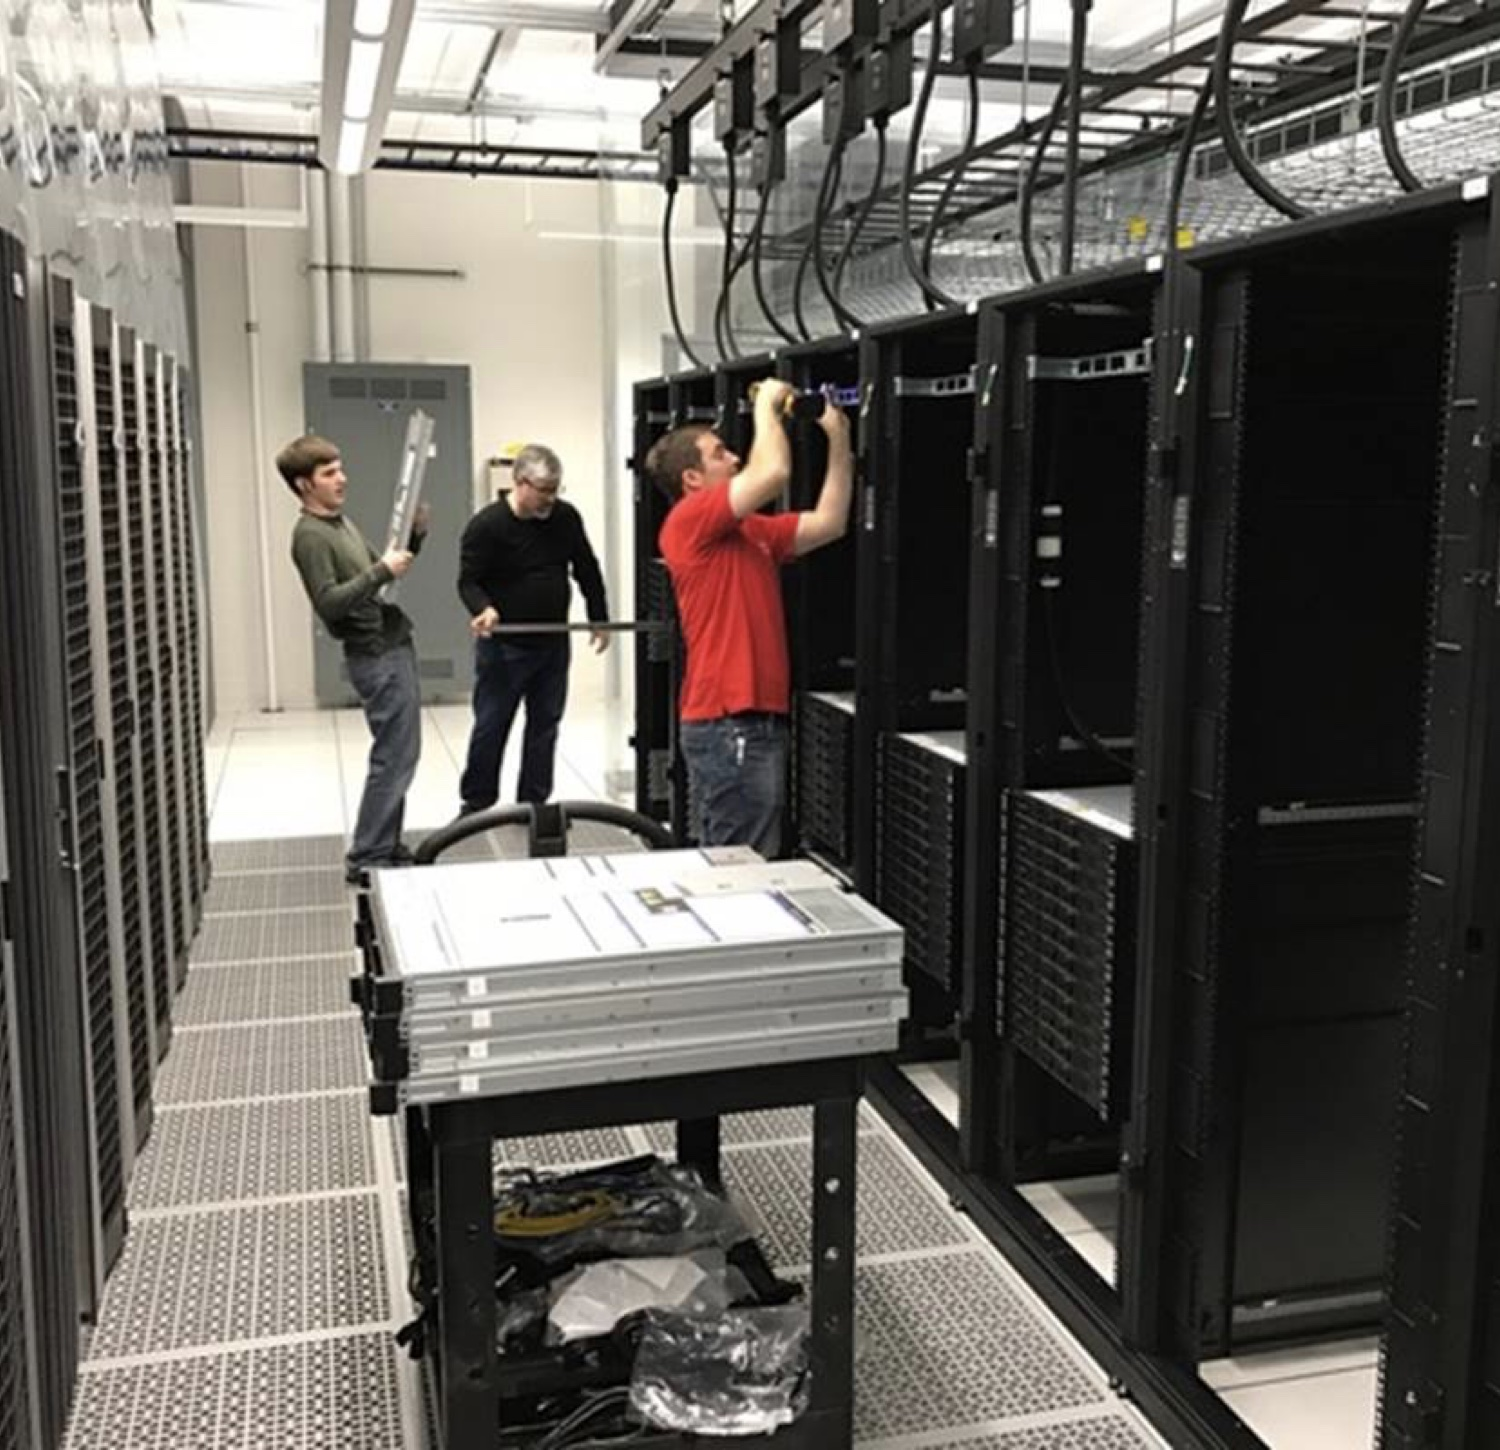
\includegraphics[width=\textwidth]{figures/m2_1.jpg}
\end{center}
\end{column}
\begin{column}{0.5\textwidth}
\begin{center}
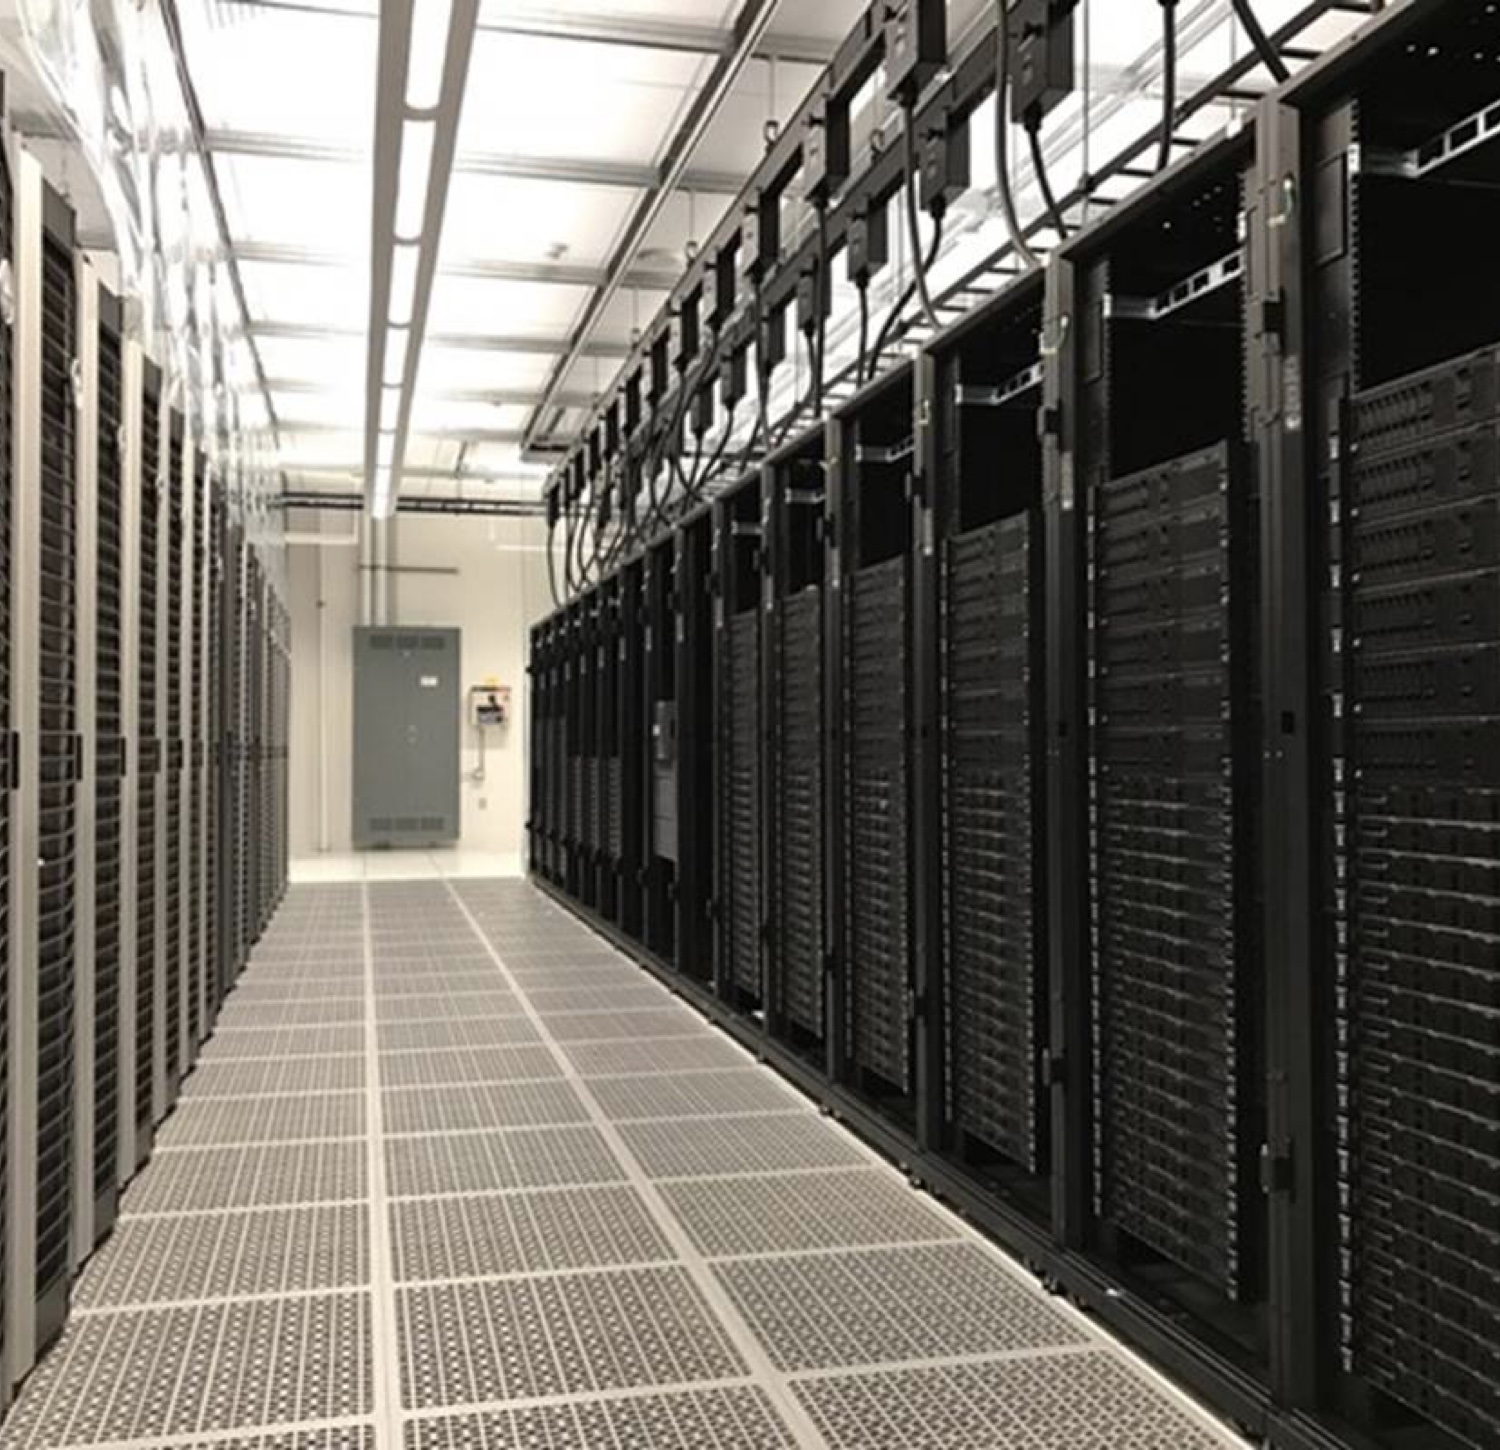
\includegraphics[width=\textwidth]{figures/m2_2.jpg}
\end{center}
\end{column}
\end{columns}
\end{frame}

\begin{frame}{Hot Aisle Containment}
\begin{columns}
\begin{column}{0.5\textwidth}
\begin{center}
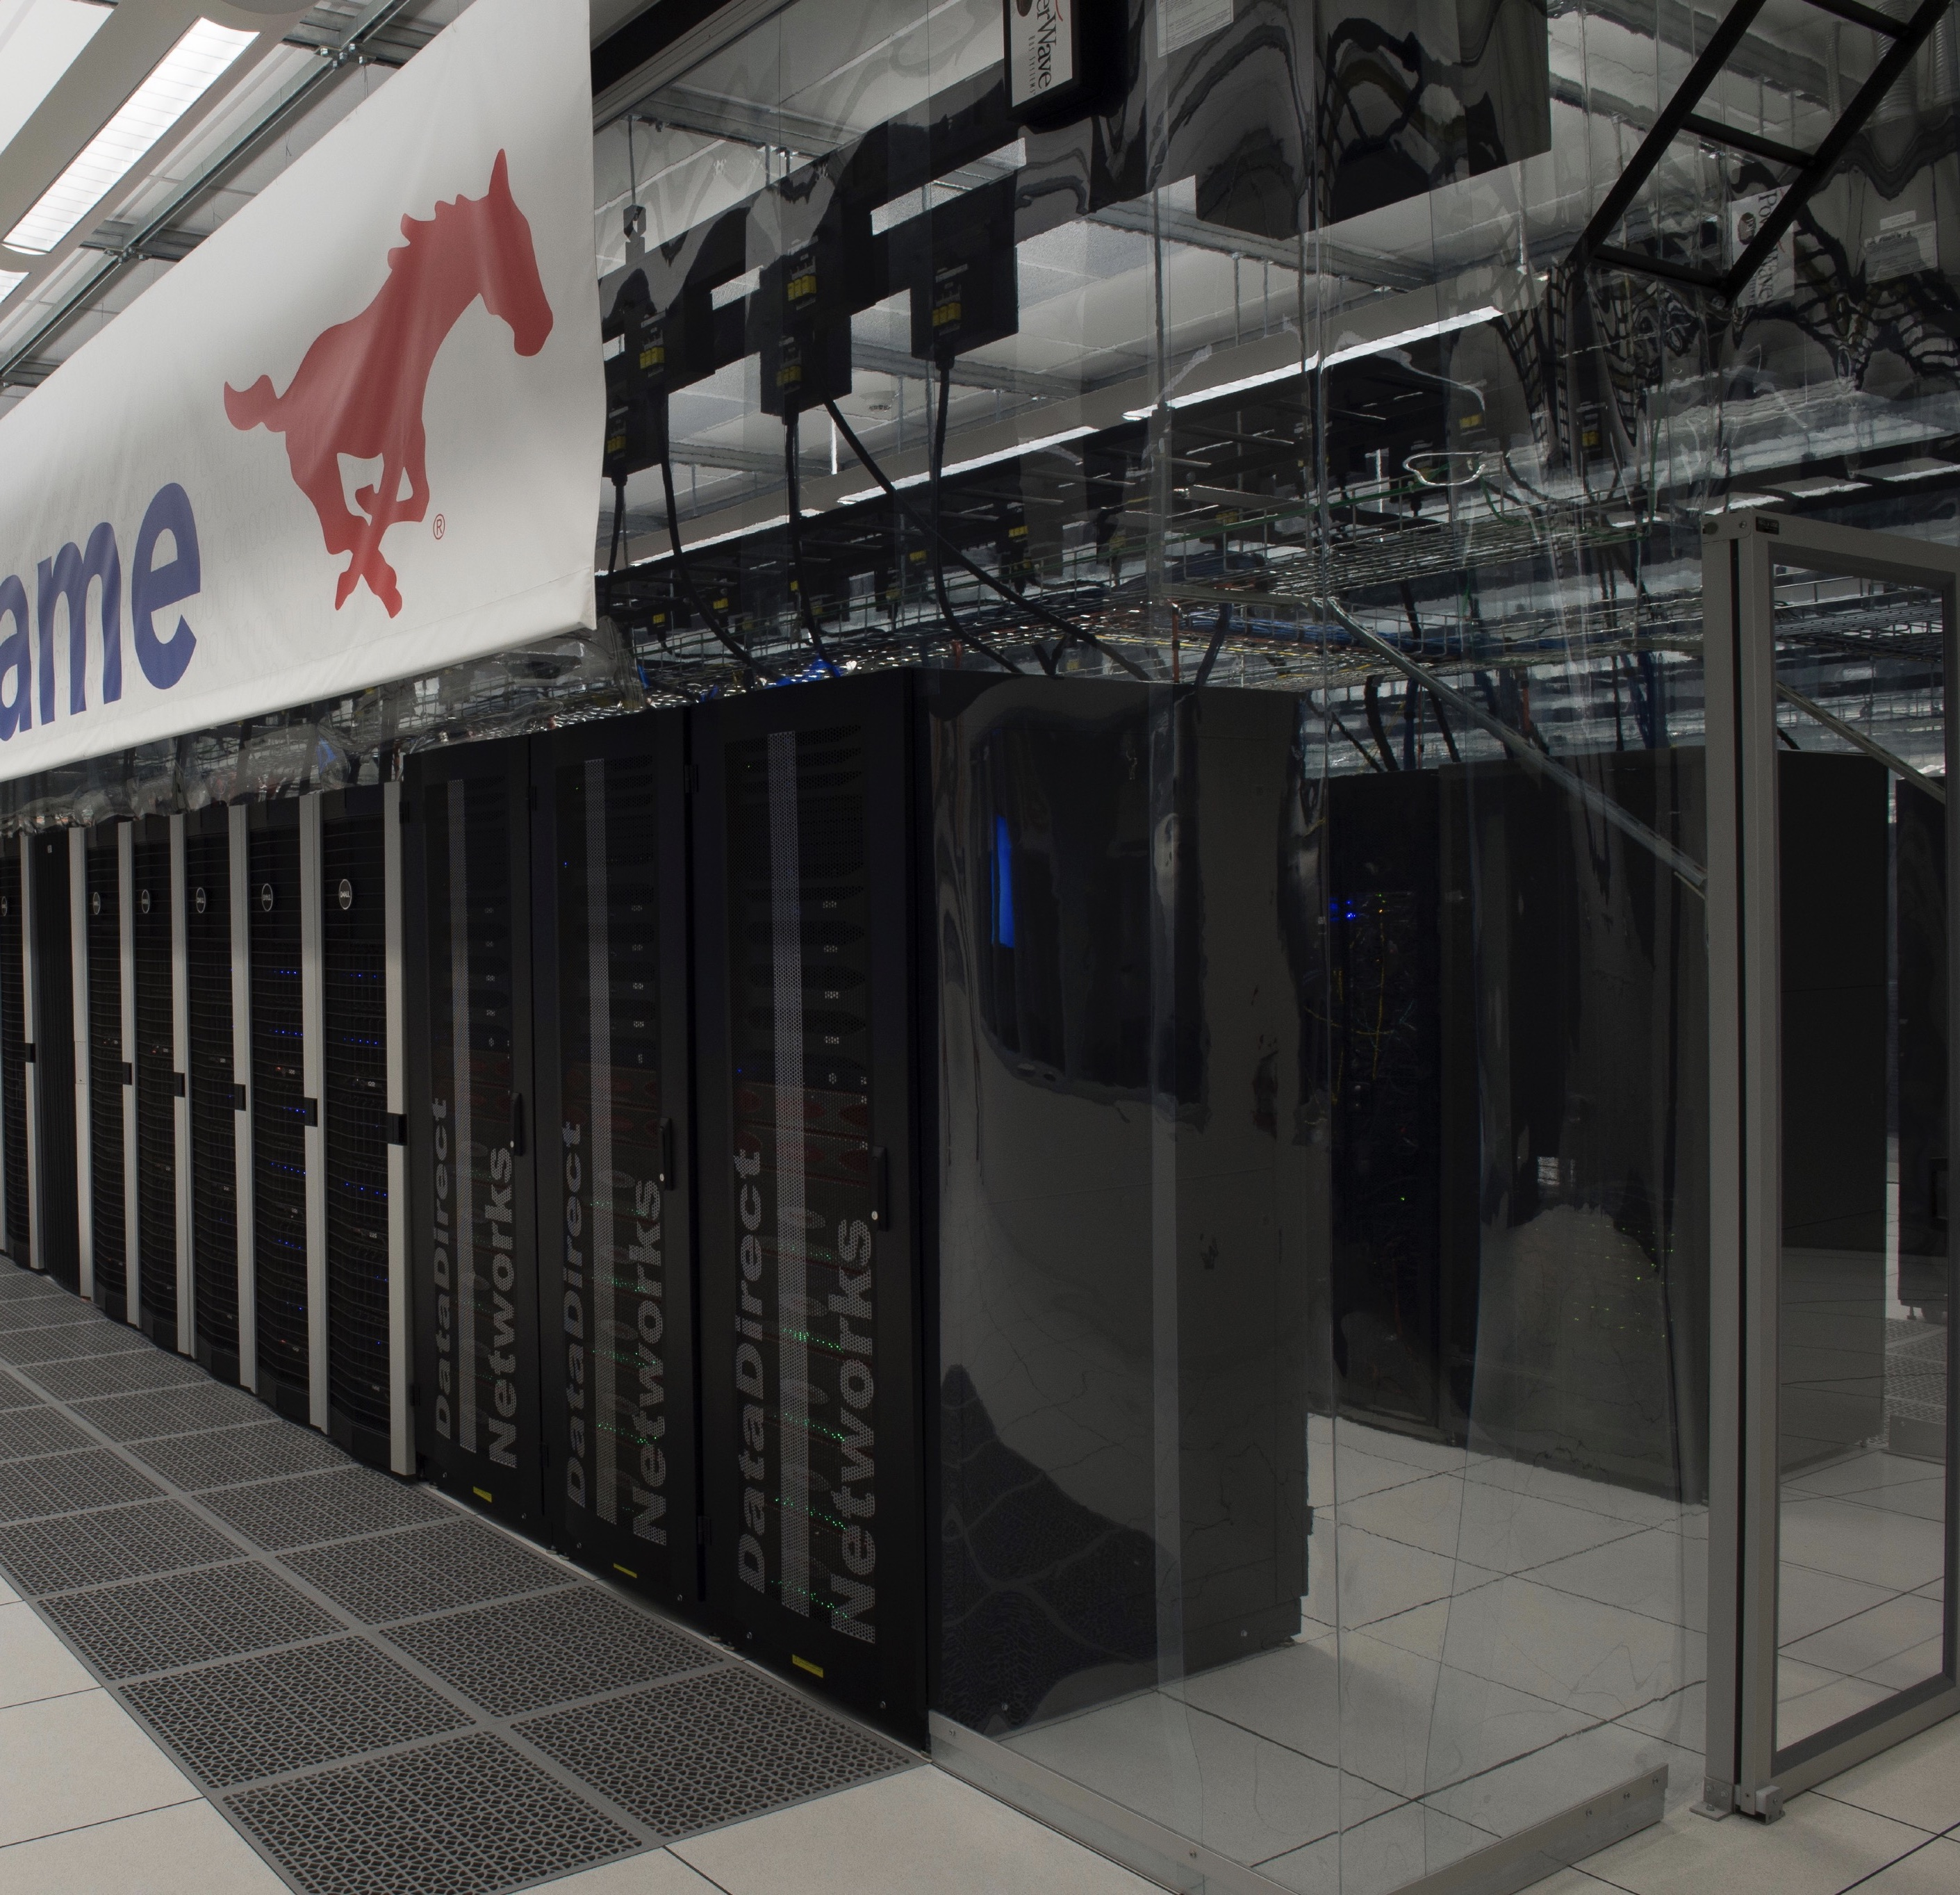
\includegraphics[width=\textwidth]{figures/hot_aisle_1.jpg}
\end{center}
\end{column}
\begin{column}{0.5\textwidth}
\begin{center}
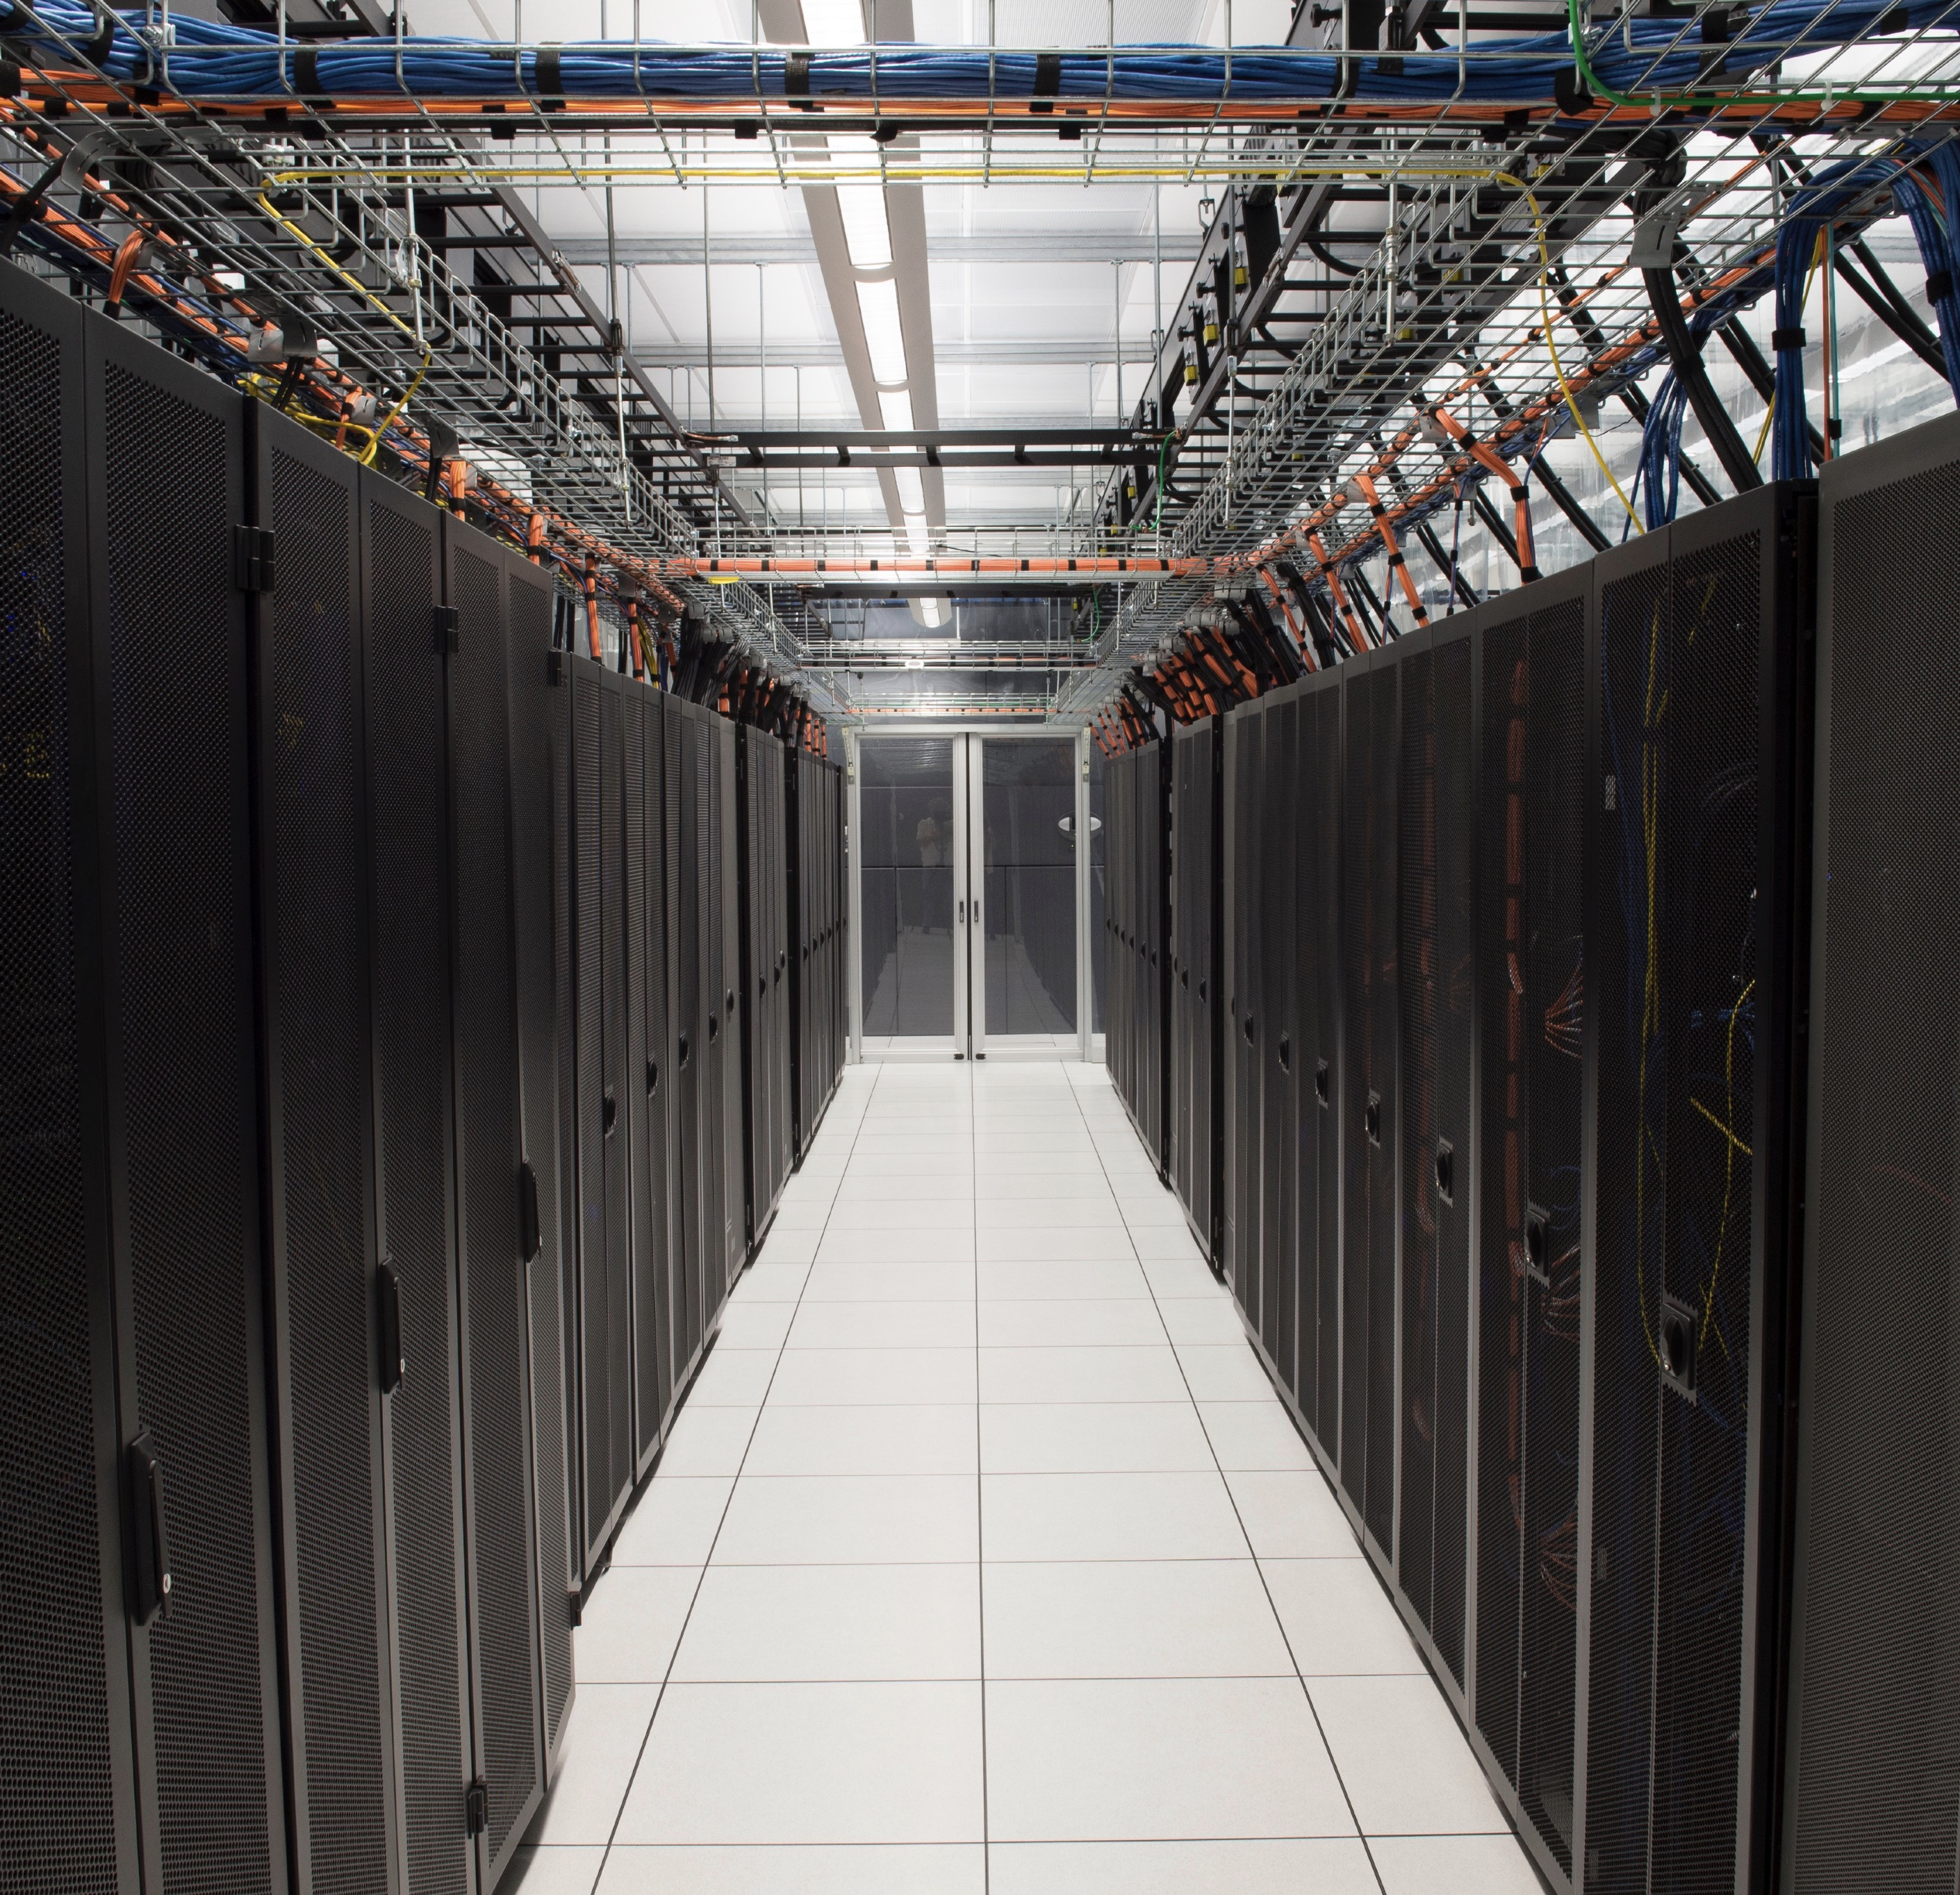
\includegraphics[width=\textwidth]{figures/hot_aisle_2.jpg}
\end{center}
\end{column}
\end{columns}
\end{frame}

\begin{frame}{Cooling and Power}
\begin{columns}
\begin{column}{0.5\textwidth}
\begin{center}
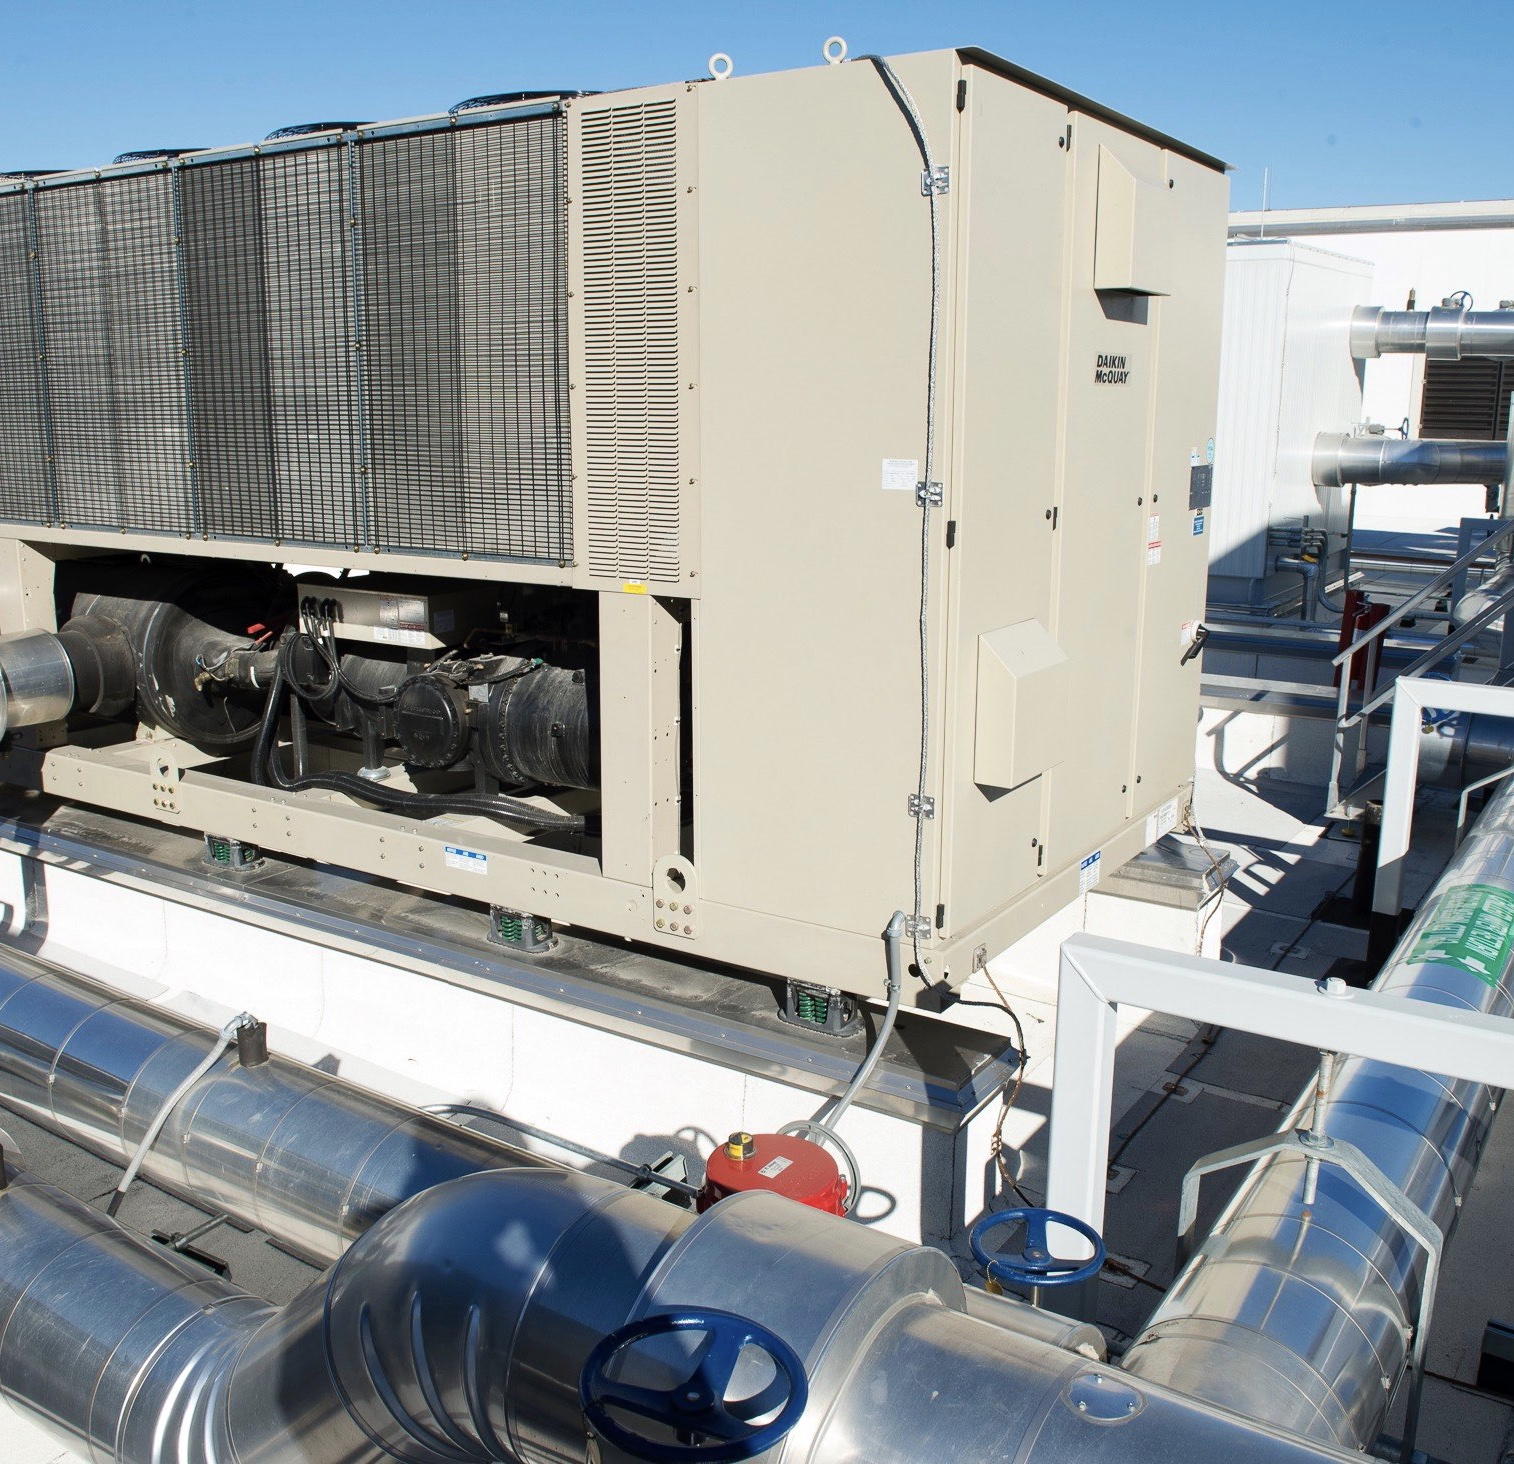
\includegraphics[width=\textwidth]{figures/cooling.jpg}
\end{center}
\end{column}
\begin{column}{0.5\textwidth}
\begin{center}
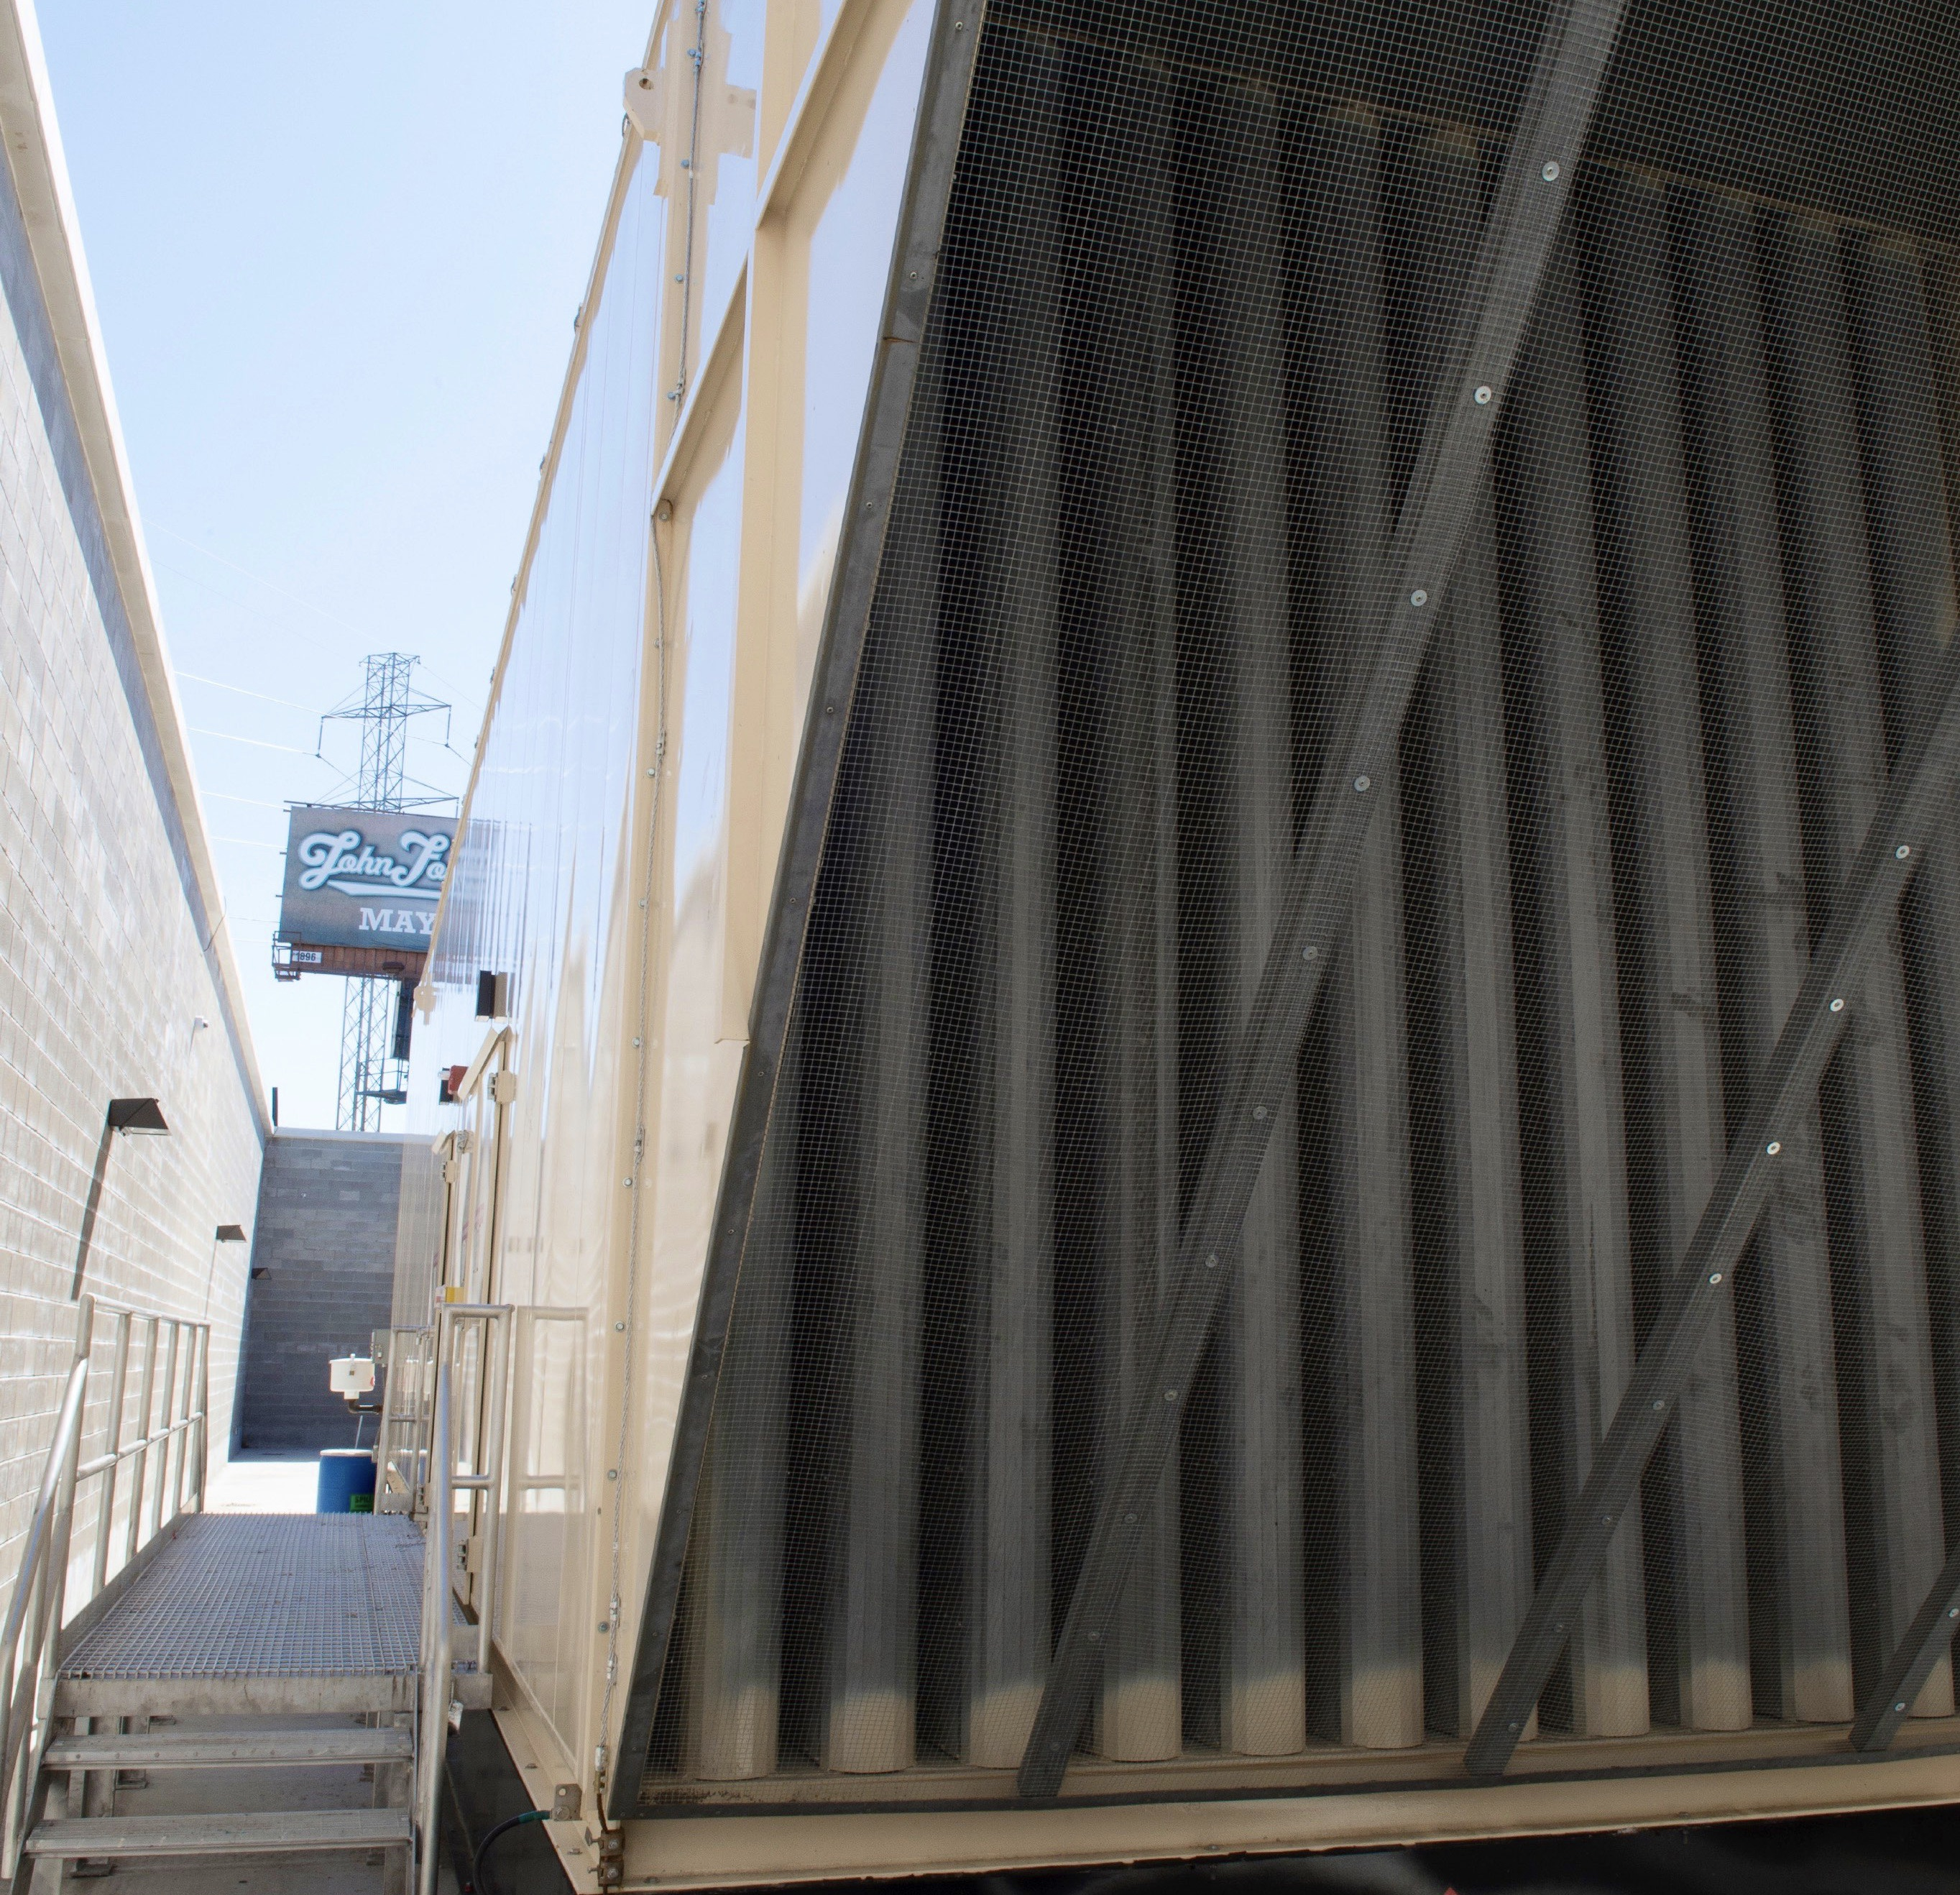
\includegraphics[width=\textwidth]{figures/power.jpg}
\end{center}
\end{column}
\end{columns}
\end{frame}

